\documentclass{article}

\usepackage{url}
\usepackage[hmargin=1.5in]{geometry}
\usepackage{enumitem}
\usepackage{amsmath}
\usepackage{amssymb}
\usepackage{amsthm}
\usepackage{eqnarray}
\usepackage{graphicx}
\usepackage[svgnames]{xcolor} %% for revisions
\usepackage{xparse} %% for squiggly underlines
\usepackage{tikz-cd} %% for term norm scratch work
\usepackage{tikz}

% TikZ libraries
\usetikzlibrary{bbox}
\usetikzlibrary{fadings}

% hat tip TeX.SE user Andrew Stacey
%   https://tex.stackexchange.com/a/82503/6934
%   https://tex.stackexchange.com/questions/82425/tikz-radial-shading-of-a-ring#comment176908_82503
\pgfdeclareradialshading{radialedge}{\pgfpointorigin}{%
  color(0bp)=(transparent!0);
  color(20bp)=(transparent!0);
  color(22bp)=(transparent!10);
  color(24bp)=(transparent!90);
  color(25bp)=(transparent!100)
}
\pgfdeclarefading{radial edge}{\pgfuseshading{radialedge}}%

%%\theoremstyle{definition}
\newtheorem{defn}{Definition}
\theoremstyle{plain}
\newtheorem{prop}{Proposition}
\newtheorem{lemma}{Lemma}
\newtheorem{thm}{Theorem}
\newtheorem{rmk}{Remark}
\newtheorem{cor}{Corollary}

% list formatting
\setlist[itemize]{leftmargin=24mm, rightmargin=12mm}
\makeatletter
% hat tip TeX.SE user31729
%   https://tex.stackexchange.com/a/328393/6934
\newcommand{\cond}[1]{\item[(\textsc{#1})]\protected@edef\@currentlabel{\textsc{#1}}}
\newcommand{\condconst}[2]{\item[($\text{\textsc{#1}} \mid #2$)]\protected@edef\@currentlabel{$\text{\textsc{#1}} \mid #2$}}
\makeatother

% convenience aliases
\newcommand{\maps}{\colon}

% group action
\newcommand{\acts}{\mathbin{\raisebox{\depth}{\rotatebox{-90}{$\circlearrowright$}}}}

% symbology
\newcommand{\Z}{\mathbb{Z}}
\newcommand{\R}{\mathbb{R}}
\newcommand{\C}{\mathbb{C}}
\let\Re\relax
\DeclareMathOperator{\Re}{Re}
\newcommand{\laplace}{\mathcal{L}}
\newcommand{\series}[1]{\tilde{#1}}
\newcommand{\fracderiv}[3]{\partial^{#1}_{#2, #3}}

% function spaces
\newcommand{\cont}{\mathcal{C}}
\newcommand{\holo}{\mathcal{H}}
\newcommand{\singexp}[2]{\mathcal{H}L^\infty_{#1, #2}}
\newcommand{\singexpalg}[1]{\singexp{#1}{\bullet}}
\newcommand{\holoL}[1]{\mathcal{H}L^{#1}} %% may no longer be needed
\newcommand{\expHoloL}[2]{\mathcal{H}L^{#1}_{#2}} %% may no longer be needed

% operator under consideration
\newcommand{\volterra}{\mathcal{V}}
\newcommand{\hardpart}{\mathcal{V}_0}
\newcommand{\softpart}{\mathcal{V}_\star}
\newcommand{\hardker}{k_0}
\newcommand{\softker}{k_\star}
\newcommand{\solwhole}{f}
\newcommand{\solproto}{f_0}
\newcommand{\solptb}{f_\star}

% domain
\newcommand{\domain}{\Omega}
\newcommand{\near}{\Omega_\text{near}}
\newcommand{\far}{\Omega_\text{far}}

% drafting environments
\newenvironment{verify}{\color{ForestGreen}}{\color{black}}
\newenvironment{brainstorm}{\color{violet}\begin{itemize}}{\end{itemize}\color{black}}

\title{Regular singular Volterra equations on complex domains}
\author{Veronica Fantini and Aaron Fenyes}
\date{}

\begin{document}
\maketitle
\begin{brainstorm}
\item \textcolor{gray}{\textit{(Aaron)} State Lemma~\ref{lem:perturbed_volterra} just the way we want it.}
\begin{itemize}
    \item Proofread and drop old version.
\end{itemize}
\item \textcolor{gray}{\textit{(Aaron)} Finish introduction}
\begin{itemize}
\item \textcolor{gray}{\textit{(Veronica)} Brainstorm: what are we trying to say in this paper? Write ideas in the to-do list at the bottom of the motivation section.}
\item \textit{(Veronica)} Revise introduction, if desired.
\end{itemize}
\color{gray}
\item \textit{(Veronica)} Say in Section~\ref{setting:perturbed} that $\volterra = \hardpart + \softpart$ and write arguments we need for bounds on whole kernel (for example, in Equation~\ref{near-limit}.
\color{gray}
\item \textit{(Veronica)} Review old blue text in Section~\ref{setting:perturbed} and decide whether we want to keep any of it. Can drop unilaterally. 
\color{violet}
\item Revise stuff related to proof of main results.
\begin{itemize}
        \item \textcolor{gray}{\textit{(Aaron)} Add proof of Lemma~\ref{lem:perturbed_volterra} to Section~\ref{sec:existence and uniqueness}}
        \item \textit{(Aaron)} Revise proof of Theorem~\ref{thm:general_volterra} in Section~\ref{sec:existence and uniqueness}
        \item \textit{(Aaron)} State the desired result of Section~\ref{sec:image under soft_part}.
        \color{gray}
        \item \textit{(Veronica)} Add motivation to Section~\ref{sec:image under soft_part}, explaining that the desired result of the section follows from a more general result about the smoothing effect of $\softpart$ (Proposition~\ref{prop:smoothing}). \textcolor{green}{I added a Corollary to explicitly write how Proposition \ref{prop:smoothing} implies the regularity we want for $\softpart f_0$}
        \color{violet}
        \item \textbf{(Aaron)} Confirm again that removed $\tau+\epsilon$ upper bound on $\rho$ was unnecessary.
\end{itemize}
\item Revise text around main results.
\begin{itemize}
    \item \textcolor{gray}{Decide whether to keep Lemma~\ref{lem:perturbed_volterra} as a lemma, or to make it a theorem, and make Theorem~\ref{thm:general_volterra} its corollary. Change order as appropriate.} \textcolor{purple}{Keep Lemma~\ref{lem:perturbed_volterra} as a lemma. State it after Theorem~\ref{thm:general_volterra}.}
    \color{gray}
    \item \textit{(Veronica)} Convert ``proof'' blocks to plain prose after main results. 
\end{itemize}
\color{gray}
\item \textbf{(Veronica)} Edit statement of Theorem~\ref{thm:example} 
\begin{itemize}
    \item Edit or remove statements about making $\Lambda$ big enough
    \item Figure out how to clean up $Q(-\zeta')$ business
\end{itemize}
\color{violet}
\item Start finalizing notation for the two parts of the operator and the two parts of the solution.
\begin{itemize}
    \item \textcolor{gray}{Choose subscripts or decorations to tell things apart in equations.} Change $\hardpart$ with $\volterra_0$ and $\softpart$ with $\volterra_\star$. Same for $\hardker$ and $\softker$. 
    \item Choose names to tell things apart in prose. Currently using ``prototypical operator,'' ``prototype solution.'' Come up with names for perturbation stuff.
\end{itemize}
\item \textbf{(Aaron)} Read through Section~\ref{sec:example}.
\color{gray}
\item \textbf{(Veronica)} Consider revising notation for roots. 
\begin{itemize}
\item ``$P$ is a monic degree-$d$ polynomial with only simple zeros;''
\item ``$Q$ is a degree-$(d-1)$ polynomial, and $Q(-\alpha) \neq 0$ for for every zero $-\alpha$ of $P$;''---or even say it without formulas.
\end{itemize}
\color{violet}
\item \textbf{(Aaron)} Change list formatting so that extra indentation applies only to conditions. We're using the \texttt{enumitem} package.
\item Work on acknowledgements
\begin{itemize}
\item \textbf{(Aaron)} Add people Aaron had conversations with
\item \textbf{(Aaron)} Think about rephrasing FMHJ acknowledgement (ERC one can't be changed).
\end{itemize}
\item Reconsider using $\lesssim$ (but still leaning not to)
\begin{itemize}
    \item \textbf{(Aaron)} As an example, show how we could rewrite the argument in proof of Proposition~\ref{prop:asymptotic at infinity} with $\lesssim$.
\end{itemize}
\end{brainstorm}
\section{Introduction}
\subsection{Motivation}\label{motivation}
In its most basic form, the Laplace transform $\laplace$ turns exponential-type functions of a real ``position'' variable $\zeta$ into holomorphic\begin{verify}\footnote{\begin{verify}Suppose the magnitude of the Laplace transform integrand is Riemann-integrable on $(0, \infty)$. Write $z$ in terms of its real and imaginary parts as $x + iy$. Since the integrand is holomorphic with respect to $z$, the operator $\frac{\partial}{\partial\overline{z}} = \frac{1}{2}\left(\frac{\partial}{\partial x} + i\frac{\partial}{\partial x}\right)$ annihilates it. Using the comparison version of Leibniz's rule for improper integrals (Theorem~11.10 of A First Course in Real Analysis, by Protter and Morrey) with $\frac{\partial}{\partial x}$ and $\frac{\partial}{\partial y}$, we see that $\frac{\partial}{\partial\overline{z}}$ annihilates the whole integral.\end{verify}}\end{verify} functions of a complex ``frequency'' variable $z$. Through identities like
\begin{align*}
\frac{\partial}{\partial z} \laplace \varphi & = \laplace(z\varphi) \\
\laplace k\;\laplace \varphi & = \laplace(k * \varphi) \\
z^{-\lambda} \laplace \varphi & = \laplace\,\partial^{-\lambda} \varphi,
\end{align*}
where $\partial^{-\lambda}$ is the Riemann-Liouville fractional integral of order $\lambda \in (0, \infty)$, the Laplace transform pulls differential operators on the frequency domain back to Volterra integral operators on the position domain. The favorable regularity properties and comprehensive theory of Volterra equations can thus be brought to bear on differential equations.

Some differential equations pull back to Volterra equations with real-analytic kernels, which extend to holomorphic Volterra equations on complex extensions of the position domain. Solutions that look unrelated in the frequency domain may turn out to be linked by analytic continuation along the complex position domain, as seen in the phenomenon of {\em resurgence} \textcolor{orange}{\cite{EcalleIII}\cite{lectures-marino} \cite[Section 2.4]{sternin1995borel}}.

Differential equations with irregular singularities in the frequency domain can pull back to Volterra equations with regular singularities in the position domain. In Section~\ref{sec:example}, we'll see this helpful behavior in the class of differential equations that Ecalle calls {\em level $1$}, which includes classical examples like the modified Bessel equation, the equations describing the vibration modes of beams that taper in certain ways \textcolor{orange}{[find citation]}, and the Airy equation after a change of coordinate. This last example generalizes to some level 1 equations that feature in current research, like the Airy-Lucas and higher Airy equations~\cite[Equations 3.2 and 3.8]{charbonnier22}\cite{durugo_higher}.

From our experience with solving level 1 differential equations by Borel summation, we expect each of the corresponding integral equations to have a special kind of solution when the integration base point coincides with a regular singularity. Let's say we've chosen the position variable $\zeta$ so that the integration base point is at $\zeta = 0$, and our position-domain Volterra operator has a holomorphic kernel $k(a, a')$ with a $\tau/\zeta(a)$ singularity. Assuming the residue $\tau$ is real and positive, we expect to find a solution with the following features:
\begin{itemize}
\item It has an $O\big(\zeta^{\tau-1}\big)$ singularity at $\zeta = 0$.
\item It's of exponential type, meaning that it's $O\big(e^{\Lambda|\zeta|}\big)$ for some $\Lambda \in \R$ as $\zeta$ grows.
\end{itemize}
These conditions are just strong enough to ensure that the solution has a well-defined Laplace transform, which by construction will satisfy the differential equation we started with in the frequency domain. The first condition also tells us that the Laplace-transformed solution is $O(z^{-\tau})$ as the frequency variable $z$ grows.

Our goal is to justify the expectations above with an existence and uniqueness result, stated in Section~\ref{sec:results}. We'll achieve it by embodying our expectations in a Banach space of holomorphic functions---the space $\singexp{\tau-1}{\Lambda}(\domain)$ defined in Section~\ref{fn-spaces}. We'll apply our results to level $1$ differential equations in Section~\ref{sec:example}.
\subsection{Notation for uniform bounds}
Given a complex-valued function $\varphi$ and a non-negative, real-valued function $\omega$, we'll write $\varphi \lesssim \omega$ to say that $|\varphi|$ is bounded by a constant multiple of $\omega$. Unless we say otherwise, the bound holds throughout the domain where both functions are defined.
\subsection{Setting}\label{setting}
\subsubsection{The domain}\label{setting:domain}
Throughout this paper, as described in Section~\ref{motivation}, the position variable $\zeta$ will be the standard coordinate on $\C$. Take a simply connected open set $\domain \subset \C$ that touches but doesn't contain $\zeta = 0$. We also assume:
\begin{itemize}
\cond{star}\label{cond:star} The set $\domain$ is star-shaped around $\zeta = 0$. In other words, for any $a \in \domain$, a straight path from $\zeta = 0$ to $a$ stays in $\domain$. Since $\domain$ doesn't contain $\zeta = 0$, we'll always leave that starting point out of the path.
\end{itemize}
For the applications we have in mind, $\domain$ might look something like the set pictured below, which satisfies Condition~\eqref{cond:star}.
\begin{center}
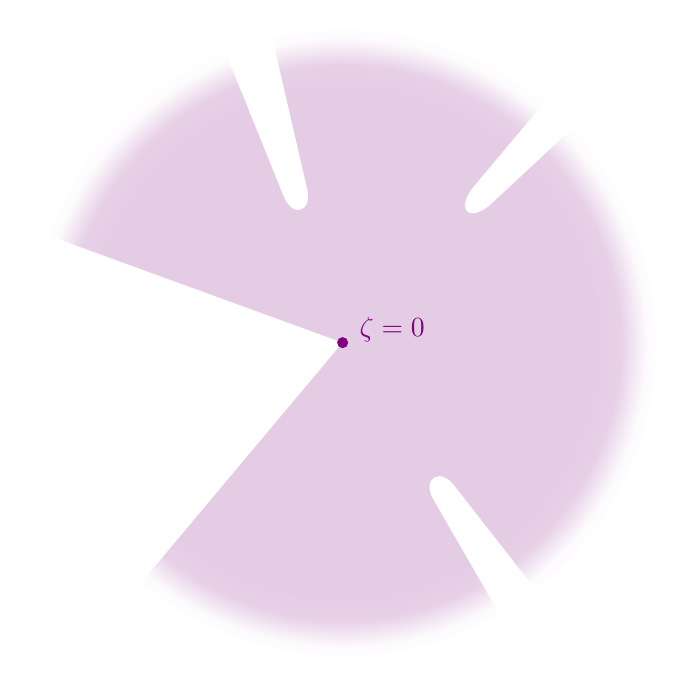
\begin{tikzpicture}
\newcommand{\spill}{4}
\fill[violet!20, bezier bounding box, path fading=radial edge]
  (-\spill, -\spill) (\spill, \spill)
  (0, 0) -- (160:\spill)
  arc (160:112:\spill) -- (112:2) .. controls (112:1.7) and (103:1.7) .. (103:2) -- (103:\spill)
  arc (103:50:\spill) -- (50:2.6) .. controls (50:2.2) and (43:2.2) .. (43:2.6) -- (43:\spill)
  arc (43:-52:\spill) -- (-52:2.3) .. controls (-52:2) and (-60:2) .. (-60:2.3) -- (-60:\spill)
  arc (-60:-130:\spill) -- (0, 0);
\fill[violet] circle (0.7mm) node[anchor=195, outer sep=1mm] {$\zeta = 0$};
\end{tikzpicture}
\end{center}
\subsubsection{The prototype operator}\label{setting:basic}
The prototypical example of the kind of operator we'll be working with is a holomorphic Volterra operator $\hardpart$ with a separable kernel and a regular singularity at $\zeta = 0$.

Being a holomorphic Volterra operator means that $\hardpart$ sends each holomorphic function $\varphi$ on $\domain$ to a new holomorphic function
\[ [\hardpart\,\varphi](a) = \int_{\zeta = 0}^a \hardker(a, \cdot)\,\varphi\;d\zeta. \]
Being separable means that the kernel $\hardker(a, a')$ factors into a function of $a$ times a function of $a'$. We'll suppose this product can be written as a ratio
\[ \hardker(a, a') = - \frac{q(a')}{p(a)}, \]
where $p$ and $q$ are holomorphic functions on $\domain$. Having a regular singularity at $\zeta = 0$ means the following:
\begin{itemize}
\condconst{sing}{\tau}\label{cond:sing} For some non-zero constant $\tau$---the {\em residue} of the singularity---the difference
\[ \hardker(a, a') - \frac{\tau}{\zeta(a)} \]
is bounded on a neighborhood of $\big(\zeta(a), \zeta(a')\big) = (0, 0)$ in $\domain^2$.
\end{itemize}
We'll assume that $\tau$ is real and positive.

Our definition of a regular singularity implies that as $|\zeta|$ goes to zero, $|p|$ also goes to zero, while $|q|$ settles into a compact interval that doesn't include zero.
\begin{verify}
[\textit{Proof.} Fix any $a'$ in the neighborhood where the difference above is bounded. By confining $a$ to small enough neighborhoods of $\zeta = 0$, we can make $|\tau/\zeta(a)|$ arbitrarily large, forcing $|q(a')/p(a)|$ to become arbitrarily large to satisfy the definition. Since $a'$ is fixed, the only way for this ratio to get arbitrarily large is for $|p(a)|$ to get arbitrarily small.]
\end{verify}
For some of our results, we'll also need to control $|p|$ and $|q|$ in various ways as $|\zeta|$ goes to infinity.
\begin{itemize}
\condconst{slow}{\lambda_0}\label{cond:slow} We can find constants $\lambda_p$ and $\lambda_\text{ratio}$ with
\begin{align*}
\left|\frac{1}{p}\right| & \lesssim e^{\lambda_p |\zeta|} &
\left|\frac{q}{p}\right| & \le \lambda_\text{ratio}
\end{align*}
outside some neighborhood of $\zeta = 0$ in $\Omega$. Note that this only constrains the ratio of $p$ and $q$ when they're evaluated at the same point. The constants will only enter our reasoning through their sum, $\lambda_0 = \lambda_p + \lambda_\text{ratio}$.
\end{itemize}
This condition explains why $\domain$ might have the sort of shape illustrated in Section~\ref{setting:domain}. As $\domain$ stretches out toward infinity, it has to part around the zeros of $p$, keeping well away from every zero except the one at $\zeta = 0$.
\begin{itemize}
\condconst{diag$_0$}{\lambda_\Delta}\label{cond:diag-basic} We can find a constant $\lambda_\Delta$ with
\[ \big| \hardker(a, a') \big| \leq \,  \textcolor{magenta}{C_\Delta} e^{\lambda_\Delta|\zeta(a)-\zeta(a')|} \]
over all $a$ in $\domain$ outside some neighborhood of $\zeta = 0$, and all $a' \in \domain$.
%%outside a neighborhood of $\zeta(a) = 0$ in $\domain^2$.
\end{itemize}
\subsubsection{The perturbed operator}\label{setting:perturbed}

Now, let's perturb $\hardpart$ to a more general operator $\volterra=\hardpart +\softpart$. The perturbation $\softpart$ doesn't have a separable kernel,\footnote{Unless $\softpart$ is zero, of course.} but does have a smoothing effect that counteracts the singularity of $\hardpart$ (as we'll show in Proposition \ref{prop:smoothing}). To get the smoothing effect, we'll require the kernel $\softker$ of $\softpart$ to vanish to some order $\epsilon > 0$ on the diagonal in $\Omega^2$. This requirement, combined with two others, will be made precise in Condition~\eqref{cond:eps-lambda}.

Since $\softpart$ is a holomorphic Volterra operator, $\softker$ is a holomorphic function on $\domain^2$. We'll allow $\softker(a, a')$ to have a simple pole at $\zeta(a) = 0$, like $\hardker(a, a')$ does, but we won't allow any sharper singularity. We'll also put an exponential bound on how fast $\softker$ grows away from the diagonal, mimicking Condition~\eqref{cond:diag-basic} on $\hardker$. Altogether, we'll require:
\begin{itemize}
\condconst{diag$_\star$}{\epsilon, \lambda_\Delta}\label{cond:eps-lambda} We have
\[ \big| \softker(a, a') \big| \leq \textcolor{magenta}{C_k}\frac{|\zeta(a)-\zeta(a')|^\epsilon}{|\zeta(a)|}\,e^{\lambda_\Delta|\zeta(a)-\zeta(a')|}\]
over all $a, a' \in \domain$.
\end{itemize}
Notice that this condition prevents $\softker$ from being separable---unless it's zero, of course.

Like $\hardker$, the combined kernel $k = \hardker + \softker$ of $\volterra$ grows in a controlled way when its arguments are near $\zeta = 0$, and when the difference between its arguments grows. We'll provide specific bounds in Section~\ref{sec:bounds on k}. 

\subsection{Main results}\label{sec:results}
%%\begin{defn}\label{fin-order}
%%Consider a Volterra operator $\mathcal{V}$ of the form
%%\[ [\mathcal{V}\varphi](a) = m(a)\,\varphi(a) + \int_{\zeta = 0}^{a} k(a, \cdot)\,\varphi\,d\zeta. \]
%%We'll say $\mathcal{V}$ is {\em effectively finite-order} over a domain $\Omega$ if there are some $c, c' \in (0, \infty)$ for which
%%\begin{itemize}
%%\item $|m(a)| \lesssim e^{c|\zeta(a)|}$ over all $a \in \Omega$
%%\item $|k(a, a')| \lesssim e^{c|\zeta(a)| + c'|\zeta(a')|}$ over all $a, a' \in \Omega$
%%\end{itemize}
%%and at one of the following holds:
%%\begin{enumerate}
%%\item\label{case:0th-order} $m$ isn't the zero function.
%%\item\label{case:pos-order} $m$ is the zero function, and there's some $\lambda \in (0, \infty)$ for which
%%\[ |k(a, a')| \in O_\text{\rm diag}\big( |\zeta(a) - \zeta(a')|^{\lambda-1} \big), \]
%%where {\rm ``diag''} means the diagonal in $\Omega^2$.
%%\end{enumerate}
%%We'll say $\mathcal{V}$ has order $0$ in case~\ref{case:0th-order}, and order at least $\lambda$ in case~\ref{case:pos-order}.
%%\end{defn}
\begin{thm}\label{thm:basic_volterra}
Let $\hardpart$ be the operator described in Section~\ref{setting:basic} and assume it satisfies {\em Condition \eqref{cond:sing}}. Then the regular singular Volterra equation
\[ f = \hardpart f \]
have the {\em prototype solution}
\begin{equation}\label{eqn:test_solution}
f_0(a)=\frac{p(b)}{p(a)} \exp\left(-\int_{b}^{a}\frac{q}{p}\;d\zeta\right).
\end{equation}
Changing the base point $b \in \domain$ just multiplies $f_0$ by a non-zero constant.

The magnitude $|f_0|$ is bounded by a constant multiple of $|\zeta|^{\tau-1}$ near $\zeta = 0$.

%%The solution $f_0$ scales like $\zeta^{\tau-1}$ as $\zeta$ goes to zero. To be precise, as $\zeta$ goes to zero, $|f_0/\zeta^{\tau-1}|$ settles into a compact interval that doesn't include zero.
\end{thm}
We'll prove this result in Section~\ref{sec:proto-construction-regularity}: by Proposition~\ref{prop:construction} we show that $f_0$ is a solution, and by Proposition~\ref{prop:asymptotic at zero} we show that it scales as desired as $\zeta$ goes to zero.

\begin{rmk}
If $q$ has a limit at $\zeta = 0$, the solution $f_0$ from Theorem~\ref{thm:basic_volterra} can be written as a constant mutiple of $\zeta^{\tau-1}$ plus a function which is $O(\zeta^\tau)$ at $\zeta = 0$.

\textcolor{RoyalBlue}{$f_0 \in F\zeta^{\tau-1} + O(\zeta^\tau)$ near $\zeta = 0$ for some non-zero constant $F$.}
\end{rmk}
\begin{thm}\label{thm:proto-growth}
Suppose $\hardpart$ satisfies {\em Condition~\eqref{cond:sing}} and {\em \eqref{cond:slow}} from Section~\ref{setting:basic}. Then the solution $f_0$ from {\em Theorem~\ref{thm:basic_volterra}} is uniformly of exponential type $\lambda_0$.\footnote{Recall that a function is of exponential type $\Lambda$ if for every $\varepsilon>0$ there is a constant $A_\varepsilon$ (which depends on $\varepsilon$) such that $|f(x)|\leq A_\varepsilon e^{\Lambda+\varepsilon} $. We instead require that there exists a uniform constant $A$ such that for every $\varepsilon>0$ the bound holds.} In light of the behavior at $\zeta = 0$ described above, this tells us that $f_0$ belongs to the space $\singexp{\tau-1}{\lambda_0}(\domain)$ defined in Section~\ref{fn-spaces}.
\end{thm}

We'll prove this result in Section~\ref{sec:proto-construction-regularity}, Proposition~\ref{prop:asymptotic at infinity}.
\begin{thm}\label{thm:general_volterra}
In the perturbed operator $\volterra = \hardpart +\softpart$ from Section~\ref{setting}, suppose the prototypical part $\hardpart$ satisfies {\em Conditions \eqref{cond:sing}}, \eqref{cond:slow}, and \eqref{cond:diag-basic} from Section~\ref{setting:basic}, and the perturbation $\softpart$ satisfies Condition \eqref{cond:eps-lambda} from Section~\ref{setting:perturbed}. Then the Volterra equation
\[f = \volterra f\]
has a unique solution $f$ in the affine subspace
\[ f_0 + \singexpalg{\tau-1+\epsilon}(\Omega) \]
of the function space $\singexpalg{\tau-1}(\Omega)$ defined in Section~\ref{fn-spaces}. Here, $f_0$ is the prototype solution \eqref{eqn:test_solution} from Theorems \ref{thm:basic_volterra}--\ref{thm:proto-growth}, which belongs to the function space $\singexp{\tau-1}{\lambda_0}(\Omega)$.

For any $\rho > \tau$, the uniqueness of the solution still holds in $f_0 + \singexpalg{\rho-1}(\Omega)$. In other words, lowering $\rho$ into $(\tau, \tau+\epsilon)$ to allow a sharper singularity won't reveal any more solutions, and raising $\rho$ too high to admit the solution found in $f_0 + \singexpalg{\tau-1+\epsilon}(\Omega)$ will leave no solution at all.
\par\textcolor{RoyalBlue}{Assume $\hardpart$ satisfies {\em Conditions \eqref{cond:sing}, \eqref{cond:slow}} and {\em \eqref{cond:diag-basic}} from Section \ref{setting:basic}. Assume $\softpart$ satisfies {\em Condition \eqref{cond:eps-lambda}} from Section \ref{setting:perturbed}. Then the Volterra equation 
\[f = \left[ \hardpart + \softpart \right] f\]
admits a unique solution in the affine subspace
\[ f_0 + \singexpalg{\tau-1+\epsilon}(\Omega) \]
of the function space $\singexpalg{\tau-1}(\Omega)$, defined in Section~\ref{fn-spaces}. The function $f_0$ is the prototypical solution of \eqref{eqn:test_solution} and it belongs to the function space $\singexp{\tau-1}{\lambda_0}(\Omega)$.}
\end{thm}
\textcolor{RoyalBlue}{We'll prove this result in Sections~\ref{sec:existence and uniqueness}: using Proposition \ref{prop:smoothing} we show that $\softpart$ maps the prototype solution into a more regular function space. Then the result follows as a consequence of Lemma \ref{lem:perturbed_volterra}.}\par
%--------
This result will follow from a more general result about inhomogeneous equations.
\begin{lemma}\label{lem:perturbed_volterra}
In the perturbed operator $\volterra = \hardpart +\softpart$ from Section~\ref{setting}, suppose the prototypical part $\hardpart$ satisfies {\em Conditions \eqref{cond:sing}} and \eqref{cond:diag-basic} \textcolor{magenta}{[I don't think we actually use \texttt{cond:slow}]} from Section~\ref{setting:basic}, and the perturbation $\softpart$ satisfies {\em Condition \eqref{cond:eps-lambda}} from Section~\ref{setting:perturbed}. Suppose we're also given a function $g$, which for some $\rho > \tau$ belongs to the space $\singexpalg{\rho-1}(\Omega)$ defined in Section~\ref{fn-spaces}. Then the inhomogeneous Volterra equation
\[ f = \volterra f + g, \]
has a unique solution $f$ in the space $\singexpalg{\rho-1}(\Omega)$.

\textcolor{RoyalBlue}{Let $g$ be a function in the space $\in\singexp{\sigma+\epsilon}{A}(\Omega)$ defined in Section~\ref{fn-spaces}. The Volterra equation
\[ f = \Big[\hardpart +\softpart \Big] f + g \]
given by an operator of the kind described in Sections \ref{setting:basic} and \ref{setting:perturbed}, admits a unique solution $f$ that belongs to $\singexp{\sigma+\epsilon}{\Lambda}(\Omega)$, for every $\Lambda\geq A$ \textcolor{magenta}{[check]}.}
\end{lemma}
\textcolor{RoyalBlue}{We'll prove this result in Section~\ref{sec:V is a contraction}: in Proposition \ref{prop:get-contraction} we construct the functions space where $\volterra$ is a contraction. Then the result follows by the contraction mapping theorem.}\par
%---------
We will prove Lemma~\ref{lem:perturbed_volterra} in Sections \ref{sec:V is a contraction}--\ref{sec:existence and uniqueness}, using the contraction mapping theorem. The heart of the argument is Proposition~\ref{prop:get-contraction}, which shows us how to find relevant subspaces where $\volterra$ is a contraction.

We will reduce Theorem~\ref{thm:general_volterra} to Lemma~\ref{lem:perturbed_volterra} in Section~\ref{sec:existence and uniqueness}, by rewriting the homogeneous equation we want to solve as an inhomogeneous equation in a more regular function space. To show that the inhomogeneous term, $\softpart f_0$, is regular enough, we use Proposition~\ref{prop:smoothing} from Section~\ref{sec:image under soft_part} to show that $\softpart$ improves on the regularity of $f_0$ described by Theorem~\ref{thm:proto-growth}.

%%To prove Theorem~\ref{thm:general_volterra}, we will rewrite the homogeneous equation we want to solve as an inhomogeneous one, with $\softpart f_0$ as the inhomogeneous term.

%%We will reduce Theorem~\ref{thm:general_volterra} to Lemma~\ref{lem:perturbed_volterra} in Section~\ref{sec:existence and uniqueness}, with the help of Proposition~\ref{prop:smoothing} from Section~\ref{sec:image under soft_part}, which can be used to show that $\softpart f_0$ is regular enough to serve as the inhomogeneous term in the lemma.
\subsection{Acknowledgements}

This paper is a result of the ERC-SyG project, Recursive and Exact New Quantum Theory (ReNewQuantum) which received funding from the European Research Council (ERC) under the European Union's Horizon 2020 research and innovation programme under grant agreement No 810573. 

We thank Fondation Mathematique Jacques Hadamard for supporting the visit of the second author at IH\'ES, under the program \textit{Junior Scientific Visibility}.  


\section{Function spaces for holomorphic Volterra operators}\label{fn-spaces}
\subsection{Weighted holomorphic $L^\infty$ spaces}\label{sec:fn-space-defs}
Throughout this paper, as described in Section~\ref{motivation}, the ``position'' variable $\zeta$ will be the standard coordinate on $\C$. Take a simply connected open set $\Omega \subset \C$ that touches but doesn't contain $\zeta = 0$. Let $\cont(\Omega)$ be the space of continuous complex-valued functions on $\Omega$. Give $\cont(\Omega)$ the compact-open topology, recalling that this is the coarsest topology in which the seminorm $f \mapsto \sup_K |f|$ is continuous for every compact subset $K \subset \Omega$~\cite[Example~2.6 and \S 4 notes]{fnl-cpx-anal}. The holomorphic functions form a closed subspace $\holo(\Omega) \subset \cont(\Omega)$~\cite[Proposition~3.14]{fnl-cpx-anal}.

Fixing a real constant $\Lambda$, let's restrict our attention to holomorphic functions on $\Omega$ which are bounded by constant multiples of $e^{\Lambda|\zeta|}$. One might describe these functions as being uniformly of exponential type $\Lambda$. They form a space $\singexp{0}{\Lambda}(\Omega)$, which we'll equip with the norm $\|f\|_{0,\Lambda} = \sup_\Omega e^{-\Lambda|\zeta|}\,|f|$. With respect to the seminorm on $\holo(\Omega)$ given by a compact set $K \subset \Omega$, the inclusion map $\singexp{0}{\Lambda}(\Omega) \hookrightarrow \holo(\Omega)$ has norm $\sup_K e^{\Lambda |\zeta|}$. That means the inclusion is continuous.
\begin{prop}\label{exp-complete}
The space $\singexp{0}{\Lambda}(\Omega)$ is complete.
\end{prop}
\begin{proof}
Take a Cauchy sequence $f_1, f_2, f_3, \ldots \in \singexp{0}{\Lambda}(\Omega)$. The inclusion map $\singexp{0}{\Lambda}(\Omega) \hookrightarrow \holo(\Omega)$ is bounded with respect to each of the seminorms on $\holo(\Omega)$ given by $|f| \mapsto \sup_K |f|$ for compact subsets $K \subset \Omega$, so our sequence is Cauchy in $\holo(\Omega)$ too. Since $\holo(\Omega)$ is complete~\cite[Proposition~3.5]{fnl-cpx-anal},\footnote{That is, a sequence which is Cauchy in each of the seminorms on $\holo(\Omega)$ will always converge in the topology of $\holo(\Omega)$, which is the coarsest topology in which all of the seminorms are continuous.} our sequence converges to a function $f$ there.

The Cauchy property in $\singexp{0}{\Lambda}(\Omega)$ tells us that for any $r > 0$, we can find some $n$ for which $e^{-\Lambda |\zeta|}\,|f_k - f_n| \le r$ whenever $k \ge n$. Since convergence in $\holo(\Omega)$ implies pointwise convergence, we can see as $k$ grows that $e^{-\Lambda |\zeta|}\,|f - f_n| \le r$. This shows that our sequence converges to $f$ in the norm $\|\cdot\|_{0,\Lambda}$. We can also see from this argument that $f$ is in $\singexp{0}{\Lambda}$: picking some $r > 0$, we observe that
\begin{align*}
e^{-\Lambda |\zeta|}\,|f| & \le e^{-\Lambda |\zeta|}\,|f - f_n| + e^{-\Lambda |\zeta|}\,|f_n| \\
& \le r + \|f_n\|_{0,\Lambda}
\end{align*}
for the corresponding $n$, showing that $e^{-\Lambda |\zeta|}\,|f|$ is bounded.

%%We can also use the Cauchy property in $\singexp{0}{\Lambda}(\Omega)$ to bound the norms $\|f_n\|_{0,\Lambda}$ uniformly over all $n$. Then, from the pointwise convergence argument above, we can draw the additional conclusion that $f$ is in $\singexp{0}{\Lambda}(\Omega)$.
\end{proof}

Now, let's relax our norm to allow both exponential growth at infinity and a power-law singularity at $\zeta = 0$. Let $\singexp{\sigma}{\Lambda}(\Omega)$ be the space of holomorphic functions on $\Omega$ which are bounded by constant multiples of $|\zeta|^\sigma e^{\Lambda|\zeta|}$. Give it the norm $\|f\|_{\sigma,\Lambda} = \sup_\Omega |\zeta|^{-\sigma} e^{-\Lambda|\zeta|}\,|f|$. Reprising the arguments from above, we can show that the inclusion $\singexp{\sigma}{\Lambda}(\Omega) \hookrightarrow \holo(\Omega)$ is continuous, and we can generalize Proposition~\ref{exp-complete}:
\begin{prop}
The space $\singexp{\sigma}{\Lambda}(\Omega)$ is complete.
\end{prop}

\subsection{Continuous inclusions between different $\singexp{\sigma}{\Lambda}(\Omega)$}\label{sec:inclusions}
\begin{prop}\label{prop:inclus-ge-exp}
If $\Lambda'\leq\Lambda$, the inclusion map $\singexp{\sigma}{\Lambda'}(\Omega)\hookrightarrow \singexp{\sigma}{\Lambda}(\Omega)$ is continuous.
\end{prop}
\begin{proof}
By definition,
\[ \|f\|_{\sigma,\Lambda}=\sup_{\Omega} |\zeta|^{-\sigma}\,e^{-\Lambda |\zeta|}\, |f|. \]
The norm $\|\cdot\|_{\sigma, \Lambda'}$ is designed to give $|f| \le |\zeta|^\sigma\,e^{\Lambda'|\zeta|}\,\|f\|_{\sigma, \Lambda'}$, which tells us that
\begin{align*}
\|f\|_{\sigma,\Lambda} & \leq \sup_{\Omega} |\zeta|^{-\sigma}\,e^{-\Lambda |\zeta|}\,|\zeta|^\sigma\,e^{\Lambda'|\zeta|}\,\|f\|_{\sigma, \Lambda'}\\
&=\sup_{\Omega} e^{-(\Lambda-\Lambda') |\zeta|}\,\|f\|_{\sigma, \Lambda'}\\
&\leq \|f\|_{\sigma,\Lambda'}.
\end{align*}
In the last step, we use the assumption that $\Lambda' \le \Lambda$.
\end{proof}
As we mentioned in Section~\ref{sec:fn-space-defs}, one might describe $\singexp{0}{\Lambda}(\domain)$ as the space of functions on $\domain$ which are uniformly of exponential type $\Lambda$. Taking the union of these spaces over all $\Lambda \in \R$, we get the space $\singexpalg{0}$ that contains all functions of exponential type. Having continuous inclusions between the subspaces $\singexp{0}{\Lambda}(\domain)$ as $\Lambda$ increases, we can give $\singexpalg{0}$ a meaningful topology: the finest topology that makes all the inclusions $\singexp{0}{\Lambda}(\domain) \hookrightarrow \singexpalg{0}$ continuous.\footnote{In category-theoretic language, $\singexpalg{0}$ is the limit of the family $\singexp{0}{\Lambda}(\domain)$.}
\begin{prop}\label{prop:inclus-lt-pow-gt-exp}
If $\sigma'>\sigma$ and $\Lambda'<\Lambda$, the inclusion map $\singexp{\sigma'}{\Lambda'}(\Omega)\hookrightarrow \singexp{\sigma}{\Lambda}(\Omega)$ is continuous.
\end{prop}
\begin{proof}
By definition,
\begin{align*}
\|f\|_{\sigma,\Lambda}&=\sup_{\Omega} |\zeta|^{-\sigma}  e^{-\Lambda |\zeta|} |f|\\
&= \sup_{\Omega} |\zeta|^{\sigma'-\sigma}\,|\zeta|^{-\sigma'}\,e^{-\Lambda'|\zeta|}\,  e^{-(\Lambda-\Lambda') |\zeta|} \, |f|.
\end{align*}
The function $|\zeta|^{\sigma'-\sigma}\,  e^{-(\Lambda-\Lambda') |\zeta|}$ is bounded near $\zeta = 0$ because the power of $|\zeta|$ is positive, and it's bounded far from $\zeta = 0$ thanks to the decaying exponential. Hence,
\begin{align*}
\|f\|_{\sigma,\Lambda}&\leq C\sup_\Omega  |\zeta|^{-\sigma'}\, e^{-\Lambda'|\zeta|} \, |f|\\
&=C \|f\|_{\sigma',\Lambda'}
\end{align*}
for $C = \sup_{\Omega}  |\zeta|^{\sigma'-\sigma}\,  e^{-(\Lambda-\Lambda') |\zeta|}$.
\end{proof}
\begin{prop}\label{prop:inclus-lt-pow-alg}
When $\sigma' > \sigma$, there's a continuous inclusion $\singexpalg{\sigma'}(\Omega)\hookrightarrow \singexpalg{\sigma}(\Omega)$.
\end{prop}
\begin{proof}
For each $\Lambda'$, we can get a continuous inclusion $\singexp{\sigma'}{\Lambda'}(\Omega) \hookrightarrow \singexpalg{\sigma}(\Omega)$ by choosing some $\Lambda > \Lambda'$ and composing the continuous inclusion $\singexp{\sigma'}{\Lambda'}(\Omega) \hookrightarrow \singexp{\sigma}{\Lambda}(\Omega)$ given by Proposition~\ref{prop:inclus-lt-pow-gt-exp} with the continuous inclusion $\singexp{\sigma}{\Lambda}(\Omega) \hookrightarrow \singexpalg{\sigma}(\Omega)$ that we get by definition. For any $\Lambda'' < \Lambda'$, the inclusions $\singexp{\sigma'}{\Lambda''}(\Omega) \hookrightarrow \singexpalg{\sigma}(\Omega)$ and $\singexp{\sigma'}{\Lambda'}(\Omega) \hookrightarrow \singexpalg{\sigma}(\Omega)$ constructed above automatically commute with the inclusion $\singexp{\sigma'}{\Lambda''}(\Omega) \hookrightarrow \singexp{\sigma'}{\Lambda'}(\Omega)$ given by Proposition~\ref{prop:inclus-ge-exp}, because we're ultimately working in the vector space of holomorphic functions on $\Omega$. Because of how the topology on $\singexpalg{\sigma'}(\Omega)$ is defined, this gives us the desired continuous inclusion $\singexpalg{\sigma'}(\Omega)\hookrightarrow \singexpalg{\sigma}(\Omega)$.
\end{proof}

%%Let $\holoL{\infty}(\Omega)$ be the space of bounded holomorphic functions on $\Omega$ with the supremum norm $\|\cdot\|_\infty$. For any $\sigma \in \R$ and $Z \in \C$, multiplying by $\zeta^\sigma e^{\Re(Z\zeta)}$ maps $\holoL{\infty}(\Omega)$ isomorphically onto another space of holomorphic functions on $\Omega$. We'll call this space $\expHoloL{\infty, \sigma}{Z}(\Omega)$ and give it the norm $\|f\|_{\infty, \sigma; Z} = \|\zeta^{-\sigma} e^{-\Re(Z\zeta)} f\|_\infty$, so that
%%\begin{align*}
%%\holoL{\infty}(\Omega) & \to \expHoloL{\infty, \sigma}{Z}(\Omega) \\
%%\varphi & \mapsto \zeta^\sigma e^{\Re(Z\zeta)} \varphi
%%\end{align*}
%%is an isometry. More generally,
%%\begin{align*}
%%\expHoloL{\infty, \rho}{Z}(\Omega) & \to \expHoloL{\infty, \rho+\delta}{Z}(\Omega) \\
%%f & \mapsto \zeta^\delta f
%%\end{align*}
%%is an isometry for all $\rho, \delta \in \R$ and $Z \in \C$. This reduces to the previous statement when $\rho = 0$ and $Z = 0$.
%%\subsection{Graded algebra structure}
%%For each $\delta \in [0, \infty)$, the functions in $\holoL{\infty, \rho}(\Omega)$ belong to $\holoL{\infty, \rho-\delta}(\Omega)$ too, and the inclusion map $\holoL{\infty, \rho}(\Omega) \hookrightarrow \holoL{\infty, \rho-\delta}(\Omega)$ has norm $\|\zeta^\delta\|_\infty$.
%%\begin{verify}
%%\begin{align*}
%%\|f\|_{\infty, \rho+\delta, Z} & = \|\zeta^{-(\rho-\delta)} e^{-\Re(Z\zeta)} f\|_\infty \\
%%& = \|\zeta^\delta \zeta^{-\rho} e^{-\Re(Z\zeta)} f\|_\infty \\
%%& = \|\zeta^\delta\|_\infty\,\|\zeta^{-\rho} e^{-\Re(Z\zeta)} f\|_\infty & \text{(Banach algebra)} \\
%%& \le \|\zeta^\delta\|_\infty\,\|f\|_{\infty, \rho; Z}
%%\end{align*}
%%\end{verify}
%%Since $\holoL{\infty}(\Omega)$ is a Banach algebra, the function space $\expHoloL{\infty, -\infty}{Z}(\Omega) := \bigcup_{\sigma \in \R} \expHoloL{\infty, \sigma}{Z}(\Omega)$ is a graded algebra, with a different norm on each grade. For each $\rho, \delta \in \R$, multiplication by a function $m \in \holoL{\infty, \delta}(\Omega)$ gives a map $\holoL{\infty, \rho}(\Omega) \to \holoL{\infty, \rho+\delta}(\Omega)$ with norm $\|m\|_{\infty, \delta}$.
%%\subsection{Norms of effectively finite-order operators}
%%\begin{itemize}
%%\item Say $|m(a)| \lesssim e^{c|\zeta(a)|}$ over all $a \in \Omega$. For any $f \in \expHoloL{\infty, \rho}{Z}$,
%%\begin{align*}
%%\|mf\|_{\infty, \sigma; Z} =
%%\end{align*}
%%\end{itemize}

%%which is effectively finite-order over $\Omega$ in the sense of Definition~\ref{fin-order}, with order at least $1 + \epsilon$ for some $\epsilon \in (0, \infty)$.
\section{Solving holomorphic Volterra equations}
\subsection{Overview}
\begin{brainstorm}
\item Explain how we're going to prove Theorem~\ref{thm:general_volterra}.
\item Roughly follow the sections. Eventual goal: make section titles match proof steps.
\begin{itemize}
\item Link to subsections during description.
\end{itemize}
\item Rough sketch of proof story:
\begin{itemize}
    \item Construct prototype solution $f_0$. Show it's in $\singexp{\tau-1}{\lambda_0}$.
    \item Show that $\softpart$ maps $f_0$ into $\singexp{\tau-1+\varepsilon}{\Lambda}$ for $\Lambda\geq\lambda_\Delta$ (see Corollary \ref{cor:pertub_f0}).
    \item Show that $\volterra$ contracts $\singexp{\rho-1}{\Lambda}$ when $\rho > \tau$ and $\Lambda$ is big enough (done in Proposition \ref{prop:get-contraction}).
    \item Use the contraction mapping theorem to prove Lemma~\ref{lem:perturbed_volterra}, and then use that lemma to prove Theorem~\ref{thm:general_volterra}.
\end{itemize}
\end{brainstorm}
\subsection{Bounds on the perturbed kernel}\label{sec:bounds on k}
 When $\hardpart$ satisfies Condition \eqref{cond:sing} and $\softpart$ satisfies Condition \eqref{cond:eps-lambda}, we can estimate the kernel $k$ near $\zeta=0$. Let $\varepsilon>0$, we can choose $\delta$ such that for every $\zeta(a)<\delta$ and $\zeta(a') <\delta$

\[ \left\vert\hardker(a,a')-\frac{\tau}{\zeta(a)} \right\vert \leq \varepsilon\]

Then, 

\begin{align*}
    |k(a,a')&\leq |\hardker(a,a')| + |\softker(a,a')|\\
    &\leq \left\vert\hardker(a,a')-\frac{\tau}{\zeta(a)} \right\vert +\frac{\tau}{|\zeta(a)|} +\textcolor{magenta}{C_k}\frac{|\zeta(a)-\zeta(a')|^\epsilon}{|\zeta(a)|}\,e^{\lambda_\Delta|\zeta(a)-\zeta(a')|}\\
    &\leq \varepsilon +\frac{\tau}{|\zeta(a)|} + \textcolor{magenta}{C_k}\frac{(2\delta)^\epsilon}{|\zeta(a)|}\,e^{\lambda_\Delta (2\delta)}\\
    &\leq \frac{\varepsilon\delta+\tau+ \textcolor{magenta}{C_k} (2\delta)^\epsilon e^{2\delta \lambda_\Delta} }{|\zeta(a)|}
\end{align*}

The constant $\sigma:=\varepsilon\delta+\tau+ \textcolor{magenta}{C_k} (2\delta)^\epsilon e^{2\delta \lambda_\Delta} > \tau $, and by choosing $\delta$ small enough we can make $\sigma-\tau$ arbitrary small. We will use this fact in Sections \ref{sec:V is a contraction} and \ref{sec:existence and uniqueness}.

Similarly, we can estimate the kernel $k$ far from $\zeta=0$. Assuming $\hardpart$ satisfies Condition \eqref{cond:diag-basic} and $\softpart$ satisfies Condition \eqref{cond:eps-lambda}, for $|\zeta(a)|\geq \delta$ and for every $a'\in\Omega$

\begin{align*}
    |k(a,a')|&\leq |\hardker(a,a')| + |\softker(a,a')|\\
    &\leq \textcolor{magenta}{C_\Delta} e^{\lambda_\Delta |\zeta(a)-\zeta(a')|} +\textcolor{magenta}{C_k}\frac{|\zeta(a)-\zeta(a')|^\epsilon}{|\zeta(a)|}\,e^{\lambda_\Delta|\zeta(a)-\zeta(a')|}\\
    &\leq \big(\textcolor{magenta}{C_\Delta} + \textcolor{magenta}{C_k}\, \delta |\zeta(a)-\zeta(a')|^\epsilon \big) \, e^{\lambda_\Delta|\zeta(a)-\zeta(a')|}
    %&\leq  \big(\textcolor{magenta}{C_\Delta} + \textcolor{magenta}{C_k}\, |\zeta(a)|^{\epsilon-1}\left\vert 1-\frac{\zeta(a')}{\zeta(a)}\right\vert^\epsilon \big) \, e^{\lambda_\Delta|\zeta(a)-\zeta(a')|}
\end{align*}
Since the growth of $|\zeta(a)-\zeta(a')|^\epsilon$ is polynomial, we can roughly estimate it by an exponential factor like 

\[|\zeta(a)-\zeta(a')|^\epsilon\lesssim e^{\lambda_\Delta |\zeta(a)-\zeta(a')|} \]

We deduce that 

\[ |k(a,a')| \leq M\, e^{2 \lambda_\Delta |\zeta(a)-\zeta(a')|} \]

with $M= \textcolor{magenta}{C_\Delta} + \delta \textcolor{magenta}{C_k}$. 

\color{purple}If $\epsilon\in (0,1]$, we actually get a better estimate, namely 

\[ |k(a,a')| \leq M\textcolor{magenta}{(a')}\, e^{ \lambda_\Delta |\zeta(a)-\zeta(a')|} \]

with $M\textcolor{magenta}{(a')} = \textcolor{magenta}{C_\Delta} + (\delta^{\epsilon-1}+\delta |\zeta(a')|^\epsilon ) \,  \textcolor{magenta}{C_k}$.\color{black}

\begin{verify}
    \begin{align*}
        \frac{|\zeta(a)-\zeta(a')|^\epsilon}{|\zeta(a)|} & \leq \frac{|\zeta(a)|^\epsilon + |\zeta(a')|^\epsilon}{|\zeta(a)|}\\
        &= |\zeta(a)|^{\epsilon-1}+ \delta |\zeta(a')|^\epsilon\\
        &\leq \delta^{\epsilon-1}+ \delta |\zeta(a')|^\epsilon 
    \end{align*}
\end{verify}

%notice that $\left\vert 1-\frac{\zeta(a')}{\zeta(a)}\right\vert^\epsilon$ is bounded by a constant which depends on $|\zeta(a')|$ (and of course on $\delta$ and $\epsilon$)



\subsection{Construction and regularity of the prototype solution \\ \textit{(proof of Theorems~\ref{thm:basic_volterra}--\ref{thm:proto-growth})}}\label{sec:proto-construction-regularity}

\subsubsection{Construction}\label{sec:construction}

\begin{prop}\label{prop:construction}
    The function 
    \begin{equation}%%\label{eqn:test_solution}
    f_0(a)=\frac{p(b)}{p(a)} \exp\left[-\int_{b}^{a}\frac{q}{p} d\zeta\right]
   \end{equation}
is a solution of the Volterra equation $\hardpart f_0=f_0$, for some $b\in\Omega$. We call $f_0$ a prototype solution.  
\end{prop}

\begin{proof}
    Let $\psi_0(a)= \exp\left[-\int_{b}^{a}\frac{q}{p} d\zeta\right]$, then $ d \psi_0 = -\frac{q}{p} \psi_0\;d\zeta $. Hence, for every $a\in\Omega$ 
    \begin{align*}
        \big[\hardpart f_0\big](a) &= - \int_{\zeta=0}^{a} \frac{q}{p(a)} f_0 d\zeta \\
        &= - \int_{\zeta=0}^{a} \frac{q}{p(a)} \frac{p(b)}{p}\psi_0 d\zeta \\
        &= - \frac{p(b)}{p(a)}  \int_{\zeta=0}^{a} \frac{q}{p} \psi_0 d\zeta\\
        &= \frac{p(b)}{p(a)}  \int_{\zeta=0}^{a} d\psi_0  \\
    \end{align*}

    Now we claim $\lim_{a\to 0}\psi_0(a)=0$: in fact, choose some $\varepsilon>0$. By Condition~\eqref{cond:sing}, we can find $\delta>0$ such that for $|\zeta(a)|<\delta$ and $|\zeta(a')|<\delta$
\begin{equation}\label{eqn:limit_h1}
\left|\frac{q(a')}{p(a)} - \frac{\tau}{\zeta(a)}\right|<\varepsilon
\end{equation}
 % notice that $|p(a)|\leq \varepsilon$ for $|zeta(a)|\leq \delta$, while $|q(a')-\ell|\leq \varepsilon$ for $|\zeta(a')|\leq \delta$ and $\ell>0$. 
 Then, we choose $b\in\Omega$ such that $\tfrac{\delta}{2}=|\zeta(b)|$.
\begin{align*}
-\int_b^a \frac{q}{p}\;d\zeta & = \int_b^a \frac{\tau}{\zeta}\;d\zeta - \int_b^a \left( \frac{q}{p} + \frac{\tau}{\zeta} \right)\;d\zeta \\
& = \tau \log\left(\frac{\zeta(a)}{\zeta(b)}\right) - \int_b^a \left( \frac{q}{p} + \frac{\tau}{\zeta} \right)\;d\zeta
\end{align*}
Exponentiating both sides, we see that
\[ \psi_0(a) = \left(\frac{\zeta(a)}{\zeta(b)}\right)^\tau \exp\left[-\int_b^a \left( \frac{q}{p} + \frac{\tau}{\zeta} \right)\;d\zeta\right]. \]
The exponential factor is bounded between $\exp\big({-\tfrac{3}{2}\varepsilon\delta}\big)$ and $\exp\big(\tfrac{3}{2}\varepsilon\delta\big)$ for all points $a$ in our chosen neighborhood of $\zeta = 0$. We deduce that $\hardpart  f_0=f_0$. 
\end{proof}


\subsubsection{Regularity}\label{sec:asymptotics}

\begin{prop}\label{prop:asymptotic at zero}
    Let $f_0$ be the prototype solution defined in \eqref{eqn:test_solution}, then $|f_0|$ is bounded by a constant multiple of $\zeta^{\tau-1}$ near $\zeta=0$. 
\end{prop}

\begin{proof}
The proof follows the argument we use at the end of the proof of proposition \ref{prop:construction}. In particular, once we choose $\varepsilon>0$ we can choose $\delta>0$ such that for $\zeta(a)<\delta$ and $\zeta(a')<\delta$ the function

\[ \psi_0(a) = \left(\frac{\zeta(a)}{\zeta(b)}\right)^\tau \exp\left[-\int_b^a \left( \frac{q}{p} + \frac{\tau}{\zeta} \right)\;d\zeta\right]. \]

is bounded by $C_1 \, |\zeta(a)|^\tau \, \exp\big(\tfrac{3}{2}\varepsilon\delta\big)$. Therefore, assuming $b'\in\Omega$ and $q(b') \neq 0$

\begin{align*}
|f_0| &  \leq C_1 |\zeta(a)|^\tau \, \exp\big(\tfrac{3}{2}\varepsilon\delta\big) \left\vert  \frac{p(b)}{p(a)}\right\vert \\
& =  C_2 |\zeta(a)|^\tau \, \left\vert\frac{p(q)}{q(b')} \right\vert \, \left\vert \frac{q(b')}{p(a)} \zeta(a)\right\vert \, |\zeta(a)|^{-1} \\
&  \leq C_3 |\zeta(a)|^{\tau-1}.
\end{align*}

The last step uses Condition~\eqref{cond:sing}. 
\end{proof}

\begin{rmk}
   {\em Proposition \ref{prop:construction}} and {\em Proposition \ref{prop:asymptotic at zero}} together prove {\em Theorem \ref{thm:basic_volterra}}. 
\end{rmk}

%In fact, if we assume $q$ to be more regular near $\zeta=0$, we get that $|f_0|/\zeta^{\tau-1}$

\begin{prop}\label{prop:asymptotic at infinity}
    Let $b\in\domain$. Assume $\hardpart$ satisfies {\em Condition} \eqref{cond:slow}. Then the prototype solution $f_0$ constructed in {\em Proposition \ref{prop:construction}} belongs to the function space $\singexp{\tau-1}{\lambda_0}(\domain)$.
\end{prop}

\begin{rmk}
    {\em Proposition \ref{prop:asymptotic at infinity}} is an equivalent formulation of {\em Theorem \ref{thm:proto-growth}}.
\end{rmk}

\begin{proof}[Proof of Proposition~\ref{prop:asymptotic at infinity}]
We choose $\varepsilon>0$, then by Condition \eqref{cond:sing} we can choose $\delta>0$ such that for $|\zeta(a)|<\delta$ and $|\zeta(a')|<\delta$ (arguing as in the proof of Proposition \ref{prop:asymptotic at zero}) we get a uniform bound 

\[   |\zeta(a)|^{-(\tau-1)} e^{-\lambda |\zeta(a)|} |f_0(a)|\leq  C_2(\delta)\, |\zeta(a)|^{-(\tau-1)} e^{-\lambda |\zeta(a)|} |\zeta(a)|^{\tau-1} \leq C_3(\delta)
\]

Now we study the regime $|\zeta(a)|>\delta$ and $|\zeta(a')|>\delta$. Recall that in Condition \eqref{cond:slow} the constant $\lambda_0$ is the sum of two constants $\lambda_0=\lambda_p+\lambda_\text{ratio}$: $\lambda_p$ controls the growth of $p^{-1}$ at infinity, and $\lambda_\text{ratio}$ controls the growth of $p/q$ at infinity. 

In particular, 
      \begin{align*}
          |\zeta(a)|^{1-\tau} e^{-\lambda_0 |\zeta(a)|} |f_0|&\leq  |\zeta(a)|^{1-\tau} e^{-\lambda_0 |\zeta(a)|} \left\vert\frac{p(b)}{p(a)}\exp\left[-\int_{b}^{a}\frac{q}{p} d\zeta\right]\right\vert \\
          & \textcolor{magenta}{\lesssim}  |\zeta(a)|^{1-\tau} e^{-\lambda_0 |\zeta(a)|}  \, e^{\lambda_p|\zeta(a)|}\exp\left[\int_{b}^{a} \Big\vert\frac{q}{p} \Big\vert |d\zeta| \right]\\
          & \textcolor{magenta}{\lesssim}  |\zeta(a)|^{1-\tau} e^{-(\lambda-\lambda_p) |\zeta(a)|} \exp\Big[\lambda_\text{ratio} |\zeta(a)-\zeta(b)| \Big]
      \end{align*}
   which is bounded because $|\zeta(a)|>\delta$. 


\end{proof}

\subsection{How $\softpart$ perturbs the prototype solution \\ \textit{(toward Theorem~\ref{thm:general_volterra})}}\label{sec:image under soft_part}

\textcolor{orange}{[Read through and revise]} In this Section, we show that, under Condition \eqref{cond:eps-lambda}, the smoothing effect of the operator $\softpart$ regularizes the prototype solution $f_0$: recall from Section \ref{sec:asymptotics} that $f_0\in\singexp{\tau-1}{\lambda_0}(\Omega)$, then we'll show $\softpart f_0 \in\singexp{\tau-1+\epsilon}{\Lambda}(\Omega)$ for $\Lambda\geq \lambda_\Delta$. This is a consequence of a more general result (see Proposition \ref{prop:smoothing}), namely that $\softpart$ regularises functions in $\singexp{\sigma}{\Lambda}(\Omega)$ which are not too singular at $\zeta=0$.  

\begin{prop}\label{prop:smoothing}
Under {\em Condition~\eqref{cond:eps-lambda}}, the operator $\softpart$ maps
\[ \singexp{\sigma}{\Lambda}(\Omega) \to \singexp{\sigma+\epsilon}{\Lambda}(\Omega) \]
continuously for all $\Lambda\geq \lambda_{\Delta}$ and $\sigma>-1$.
\end{prop}

\begin{proof}
    Let $f\in\singexp{\sigma}{\Lambda}$,
    \begin{align*}
        |\zeta(a)|^{-(\sigma+\epsilon)} \, e^{-\Lambda |\zeta(a)|} \, \Big \vert \big[ \softpart f\big](a)\Big\vert
        &\leq |\zeta(a)|^{-(\sigma+\epsilon)}\, e^{-\Lambda |\zeta(a)|} \int_{\zeta=0}^a |\softker(a,\cdot)|\, |f| \, |d\zeta| \\
        &\leq |\zeta(a)|^{-(\sigma+\epsilon)}\, e^{-\Lambda |\zeta(a)|} \int_{\zeta=0}^a |\softker(a,\cdot)|\, |\zeta|^{\sigma}\, e^{\Lambda |\zeta|} \|f\|_{\sigma,\Lambda} \, |d\zeta| 
    \end{align*}
    By Condition~\eqref{cond:eps-lambda},
    \begin{align*}
         \int_{\zeta=0}^a |\softker(a,\cdot)|\, |\zeta|^{\sigma}\, e^{\Lambda |\zeta|} \, |d\zeta| &\leq C_k \int_{\zeta=0}^a \frac{|\zeta(a)-\zeta|^\epsilon}{|\zeta(a)|} e^{\lambda_\Delta |\zeta(a)-\zeta|} |\zeta|^{\sigma}\, e^{\Lambda|\zeta|}\;|d\zeta|\\
         &=C_k |\zeta(a)|^{\epsilon+\sigma} \int_{0}^1 (1-t)^\epsilon e^{\lambda_\Delta |\zeta(a)|(1-t)} t^{\sigma}\, e^{\Lambda|\zeta(a)| t}\;dt\\
         &=C_k |\zeta(a)|^{\epsilon+\sigma}\, e^{\lambda_\Delta |\zeta(a)|}\,  \int_{0}^1 (1-t)^\epsilon  t^{\sigma}\,e^{(\Lambda-\lambda_\Delta)|\zeta(a)| t}\;dt\\
         &\le C_k |\zeta(a)|^{\epsilon+\sigma}\, e^{\lambda_\Delta |\zeta(a)|}\,e^{(\Lambda-\lambda_\Delta)|\zeta(a)|}\int_{0}^1 (1-t)^\epsilon  t^{\sigma}\;dt.
    \end{align*}
    The last step takes advantage of the assumption that $\Lambda \ge \lambda_\Delta$. Recognizing the integral as an evaluation of the beta function, we can rewrite the bound as
    \[ \int_{\zeta=0}^a |\softker(a,\cdot)|\, |\zeta|^{\sigma}\, e^{\Lambda |\zeta|} \, |d\zeta| \le C_k |\zeta(a)|^{\epsilon+\sigma}\, e^{\Lambda |\zeta(a)|} \frac{\Gamma(\epsilon+1)\Gamma(\sigma+1)}{\Gamma(\sigma+\epsilon+2)}. \]
    Our assumptions that $\epsilon > 0$ and $\sigma > -1$ ensure that the gamma functions are well-defined. Rearranging to get
    \[ |\zeta(a)|^{-(\epsilon+\sigma)}\, e^{-\Lambda |\zeta(a)|} \int_{\zeta=0}^a |\softker(a,\cdot)|\, |\zeta|^{\sigma}\, e^{\Lambda |\zeta|} \, |d\zeta| \le C_k \frac{\Gamma(\epsilon+1)\Gamma(\sigma+1)}{\Gamma(\sigma+\epsilon+2)}, \]
    we conclude that $|\zeta(a)|^{-\sigma-\epsilon} \, e^{-\Lambda |\zeta(a)|} \, \Big \vert \big[ \softpart f\big](a)\Big\vert$ is uniformly bounded in $\domain$. 
\end{proof}

\begin{cor}\label{cor:pertub_f0}
    Let $f_0$ be the prototype solution in equation \eqref{eqn:test_solution}. If $\softpart$ satisfies {\em Condition \eqref{cond:eps-lambda}}, then $\softpart f_0\in\singexp{\tau-1+\epsilon}{\Lambda}(\Omega)$, for $\Lambda\geq \lambda_\Delta$. 
\end{cor}
\begin{proof}
    Notice that since $\tau-1>-1$ the hypothesis of Proposition \ref{prop:smoothing} are satisfied. In addition, we can choose the constant $\Lambda=\max \{\lambda_0 , \lambda_\Delta\}$. 
\end{proof}

\subsection{Showing that $\volterra$ shrinks perturbations \\ \textit{(toward Lemma~\ref{lem:perturbed_volterra})}}\label{sec:V is a contraction}
\subsubsection{Overview}
In this section, we'll prove the following proposition. %We assume $\volterra$ satisfies Conditions \eqref{cond:sing}, \eqref{cond:diag-basic} and \eqref{cond:eps-lambda}. 

\begin{prop}\label{prop:get-contraction}
Suppose that $\hardpart$ satisfies {\em Conditions \eqref{cond:sing}} and \eqref{cond:diag-basic}, and $\softpart$ satisfies {\em Condition \eqref{cond:eps-lambda}}. Then, for each $\rho > \tau$, we can ensure that $\volterra$ is a contraction of $\singexp{\rho-1}{\Lambda}$ by making $\Lambda$ big enough.
\end{prop}
\begin{rmk}
For the argument, we'll use, ``big enough'' always requires $\Lambda > \lambda_\Delta$, and may require $\Lambda \gg \lambda_\Delta$.
\end{rmk}
First, pick some $\sigma \in (\tau, \rho)$.\footnote{If you'd like, you can fix a choice of $\sigma$---for example, taking $\sigma = \frac{1}{2}(\tau + \rho)$.} By Conditions \eqref{cond:sing} and \eqref{cond:eps-lambda}, we can find a neighborhood $\near \subset \domain$ of $\zeta = 0$ with the property that
\begin{equation}\label{near-limit}
|k(a, a')| \le \frac{\sigma}{|\zeta(a)|}
\end{equation}
for all $a, a' \in \near$ (see Section \ref{sec:bounds on k}). By choosing a small enough positive radius $R$, we can take $\near$ to be the part of $\domain$ where $|\zeta| < R$. Complementarily, let $\far$ be the part of $\domain$ where $R \le |\zeta|$.


Take any function $\varphi \in \singexp{\rho}{\Lambda}(\domain)$. In Section~\ref{near-bound}, we'll bound $|\zeta|^{-(\rho-1)}\,e^{-\Lambda|\zeta|}\,|\volterra\varphi|$ by $\tfrac{\sigma}{\rho} \|\varphi\|_{\rho-1, \Lambda}$ on $\near$. In Section~\ref{far-bound}, we'll see that by making $\Lambda$ big enough, we can bound $|\zeta|^{-(\rho-1)}\,e^{-\Lambda|\zeta|}\,|\volterra\varphi|$ by an arbitrarily small constant multiple of $\|\varphi\|_{\rho-1, \Lambda}$ on $\far$. Together, these results show that $\|\volterra \varphi\|_{\rho-1, \Lambda} \le \tfrac{\sigma}{\rho} \|\varphi\|_{\rho-1, \Lambda}$ when $\Lambda$ is large enough. Since we set $\sigma < \rho$, this proves Proposition~\ref{prop:get-contraction}.
\subsubsection{First steps}\label{first-steps}
The first steps of our calculation are the same throughout $\domain$. For each $a \in \domain$, we have
\[ |\zeta(a)|^{-(\rho-1)}\,e^{-\Lambda|\zeta(a)|}\,|[\volterra\varphi](a)| \le |\zeta(a)|^{-(\rho-1)}\,e^{-\Lambda|\zeta(a)|} \int_0^{\zeta(a)} |k(a, \cdot)\,\varphi\;d\zeta| \]
for any choice of integration path.\footnote{The absolute value of a $1$-form, like $|k(a, \cdot)\,\varphi\;d\zeta|$, is a density on $\C$---a norm on tangent vectors.} The norm on $\singexp{\rho-1}{\Lambda}(\domain)$ is designed to give the bound $|\varphi| \le |\zeta|^{\rho-1}\,e^{\Lambda |\zeta|}\,\|\varphi\|_{\rho-1, \Lambda}$, so
\begin{align*}
|\zeta(a)|^{-(\rho-1)}\,e^{-\Lambda|\zeta(a)|}\,|[\volterra\varphi](a)| & \le |\zeta(a)|^{-(\rho-1)}\,e^{-\Lambda|\zeta(a)|} \int_0^{\zeta(a)} |k(a, \cdot)|\,|\zeta|^{\rho-1}\,e^{\Lambda |\zeta|}\,\|\varphi\|_{\rho-1, \Lambda}\;|d\zeta| \\
& = \|\varphi\|_{\rho-1, \Lambda} \int_0^{\zeta(a)} |k(a, \cdot)|\,\left|\frac{\zeta}{\zeta(a)}\right|^{\rho-1}\,e^{-\Lambda(|\zeta(a)| - |\zeta|)}\;|d\zeta|
\end{align*}
What we do next depends on whether $a$ is in $\near$ or $\far$.
\subsubsection{Near the origin}\label{near-bound}
Suppose that $a \in \near$. Then inequality~\eqref{near-limit} tells us that
\begin{align*}
|\zeta(a)|^{-(\rho-1)}\,e^{-\Lambda|\zeta(a)|}\,|[\volterra\varphi](a)| & \le
\|\varphi\|_{\rho-1, \Lambda} \int_0^{\zeta(a)} \frac{\sigma}{|\zeta(a)|}\,\left|\frac{\zeta}{\zeta(a)}\right|^{\rho-1}\,e^{-\Lambda(|\zeta(a)| - |\zeta|)}\;|d\zeta| \\
& \le \sigma \|\varphi\|_{\rho-1, \Lambda} \int_0^{\zeta(a)} \left|\frac{\zeta}{\zeta(a)}\right|^{\rho-1}\,e^{-\Lambda(|\zeta(a)| - |\zeta|)}\;\left|\frac{d\zeta}{\zeta(a)}\right|
\end{align*}
for any integration path that stays within $\near$. Taking advantage of the fact that $\near$ is a sector of a disk, let's use the straight path $\zeta = t \zeta(a)$, with $t \in (0, 1]$.
\begin{align*}
|\zeta(a)|^{-(\rho-1)}\,e^{-\Lambda|\zeta(a)|}\,|[\volterra\varphi](a)| & \le \sigma \|\varphi\|_{\rho-1, \Lambda} \int_0^1 t^{\rho-1}\,e^{-\Lambda |\zeta(a)|(1 - t)}\;dt \\
& \le \sigma \|\varphi\|_{\rho-1, \Lambda} \int_0^1 t^{\rho-1}\;dt \\
& = \frac{\sigma}{\rho} \|\varphi\|_{\rho-1, \Lambda}.
\end{align*}
Since we set $\sigma < \rho$, this brings us halfway to proving Proposition~\ref{prop:get-contraction}.
\subsubsection{Away from the origin}\label{far-bound}
Going back to the end of Section~\ref{first-steps}, suppose that $a \in \far$. We know from Conditions \eqref{cond:diag-basic} and \eqref{cond:eps-lambda} that we can find a constant $M$ for which
\[ |k(a, \cdot)| \le M e^{\textcolor{orange}{2}\lambda_\Delta |\zeta(a) - \zeta|} \]
for all $a \in \far$ (see Section \ref{sec:bounds on k}). Note that only the first argument of $k$ has its domain restricted; this bound holds throughout $\domain$ in the second argument. Applying this bound, we learn that
\[ |\zeta(a)|^{-(\rho-1)}\,e^{-\Lambda|\zeta(a)|}\,|[\volterra\varphi](a)| \le \|\varphi\|_{\rho-1, \Lambda} \int_0^{\zeta(a)} M e^{\textcolor{orange}{2}\lambda_\Delta |\zeta(a) - \zeta|}\,\left|\frac{\zeta}{\zeta(a)}\right|^{\rho-1}\,e^{-\Lambda(|\zeta(a)| - |\zeta|)}\;|d\zeta|. \]
Let's again use the straight integration path $\zeta = t \zeta(a)$, with $t \in (0, 1]$. Along this path, $|\zeta(a) - \zeta| = |\zeta(a)| - |\zeta|$, allowing us to combine the exponential factors in our bound:
\begin{align*}
|\zeta(a)|^{-(\rho-1)}\,e^{-\Lambda|\zeta(a)|}\,|[\volterra\varphi](a)| & \le \|\varphi\|_{\rho-1, \Lambda} \int_0^1 M e^{\textcolor{orange}{2}\lambda_\Delta |\zeta(a)|(1 - t)}\,t^{\rho-1}\,e^{-\Lambda |\zeta(a)|(1 - t)}\;dt \\
& \le M \|\varphi\|_{\rho-1, \Lambda} \int_0^1 t^{\rho-1}\,e^{-(\Lambda - \textcolor{orange}{2}\lambda_\Delta)|\zeta(a)|(1 - t)}\;dt.
\end{align*}
Let's set $\Lambda > \lambda_\Delta$, ensuring that the exponential factor shrinks as $|\zeta(a)|$ grows. Then we can make our bound uniform over all $a \in \far$, since $|\zeta(a)| \ge R$ for these points:
\[ |\zeta(a)|^{-(\rho-1)}\,e^{-\Lambda|\zeta(a)|}\,|[\volterra\varphi](a)| \le M \|\varphi\|_{\rho-1, \Lambda} \int_0^1 t^{\rho-1}\,e^{-(\Lambda - \textcolor{orange}{2}\lambda_\Delta)R(1 - t)}\;dt. \]

We can make this bound less than one, as required to show that $\volterra$ is a contraction, by increasing $\Lambda$. To see this in the trickiest case, where $\rho < 1$, it helps to look at the beginning and end of the integration separately. At the beginning---for $t \in \big(0, \tfrac{1}{5}\big]$, say---we can use a worst-case estimate on the exponential factor:
\begin{align*}
\int_0^{1/5} t^{\rho-1}\,e^{-(\Lambda - \textcolor{orange}{2} \lambda_\Delta)R(1 - t)}\;dt & \le e^{-\frac{4}{5}(\Lambda -\textcolor{orange}{2} \lambda_\Delta)R} \int_0^{1/5} t^{\rho-1}\;dt \\
& = e^{-\frac{4}{5}(\Lambda \textcolor{orange}{2} \lambda_\Delta)R}\,\tfrac{1}{\rho} \big(\tfrac{1}{5}\big)^\rho.
\end{align*}
At the end, we instead use a worst-case estimate on $t^{1-\rho}$:
\begin{align*}
\int_{1/5}^1 t^{\rho-1}\,e^{-(\Lambda - \textcolor{orange}{2}\lambda_\Delta)R(1 - t)}\;dt & \le \left\{\begin{array}{cc}(1/5)^{\rho-1} & \rho \le 1 \\ 1 & \rho \ge 1 \end{array}\right\} \int_{1/5}^1 e^{-(\Lambda -\textcolor{orange}{2} \lambda_\Delta)R(1 - t)}\;dt \\
& = \left\{\begin{array}{cc}(1/5)^{\rho-1} & \rho \le 1 \\ 1 & \rho \ge 1 \end{array}\right\} \frac{1}{(\Lambda - \textcolor{orange}{2}\lambda_\Delta)R}\left[ 1 - e^{-\tfrac{4}{5}(\Lambda - \textcolor{orange}{2}\lambda_\Delta)R} \right] \\
& \le \left\{\begin{array}{cc}(1/5)^{\rho-1} & \rho \le 1 \\ 1 & \rho \ge 1 \end{array}\right\} \frac{1}{(\Lambda - \textcolor{orange}{2}\lambda_\Delta)R}.
\end{align*}

We now know that by setting $\Lambda > \textcolor{orange}{2}\lambda_\Delta+ (1/5)^{\rho-1 R^{-1}}$ (in fact $1/5$ can be replaced by any number in $(0,1)$), we can make $|\zeta(a)|^{-(\rho-1)}\,e^{-\Lambda|\zeta(a)|}\,|[\volterra\varphi](a)|$ as small as we want over all $a \in \far$. This completes our proof of Proposition~\ref{prop:get-contraction}.
\subsection{Existence and uniqueness of the perturbed solution \\ \textit{(proof of Lemma~\ref{lem:perturbed_volterra} and Theorem~\ref{thm:general_volterra})}}\label{sec:existence and uniqueness}
\begin{proof}[Proof of Lemma~\ref{lem:perturbed_volterra}]
Choose $\Lambda$ large enough to ensure that $\volterra$ is a contraction of $\singexp{\rho-1}{\Lambda}(\Omega)$ and $g$ belongs to $\singexp{\rho-1}{\Lambda}(\Omega)$. Proposition~\ref{prop:get-contraction} guarantees that we can do the former, given our assumptions about $\volterra$ and $\rho$, and the definition of $\singexpalg{\rho-1}(\Omega)$ guarantees that we can also do the latter. Our choice of $\Lambda$ ensures that the affine map $f \mapsto \volterra f + g$ is also a contraction of $\singexp{\rho-1}{\Lambda}(\Omega)$, and thus has a unique fixed point in $\singexp{\rho-1}{\Lambda}(\Omega)$ by the contraction mapping theorem.

To see that the fixed point is still unique in the bigger space $\singexpalg{\rho-1}(\Omega)$, first recall from Proposition~\ref{prop:inclus-ge-exp} that we have inclusions $\singexp{\rho-1}{\Lambda'}(\Omega) \hookrightarrow \singexp{\rho-1}{\Lambda}(\Omega)$ for all $\Lambda' \le \Lambda$. Any fixed point in $\singexp{\rho-1}{\Lambda'}(\Omega)$ must map to the unique fixed point in $\singexp{\rho-1}{\Lambda}(\Omega)$ under this inclusion. Next, observe that for any $\Lambda'' \ge \Lambda$, the map $f \mapsto \volterra f + g$ is also a contraction of $\singexp{\rho-1}{\Lambda''}(\Omega)$. The inclusion $\singexp{\rho-1}{\Lambda}(\Omega) \hookrightarrow \singexp{\rho-1}{\Lambda''}(\Omega)$ must send the unique fixed point in the smaller space to the unique fixed point in the larger one. Together, these arguments show that the fixed point is unique in $\singexpalg{\rho-1}(\Omega)$.
\end{proof}
\begin{proof}[Proof of Theorem~\ref{thm:general_volterra}]
%\textcolor{magenta}{[we have to change the definition of $\hardker$ in \S \ref{setting:basic} in $-\frac{q(a')}{p(a)}$.]}
Start with the prototype solution $\solproto$ constructed in Theorem~\ref{thm:basic_volterra}, which satisfies the equation
\[ \solproto = \hardpart \solproto. \]
The base point for the construction can be chosen arbitrarily. Under our assumptions about $\volterra$, Theorem~\ref{thm:proto-growth} tells us that $\solproto$ is in $\singexp{\tau-1}{\lambda_0}(\Omega)$. Our goal is to find a perturbation $\solptb \in \singexpalg{\tau-1+\epsilon}(\Omega)$ that makes $\solwhole = \solproto + \solptb$ a solution of
\begin{equation}\label{eqn:orig-homog}
\solwhole = \volterra \solwhole.
\end{equation}
Observing that
\begin{align*}
\volterra \solproto & = \hardpart\solproto + \softpart\solproto \\
& = \solproto + \softpart \solproto,
\end{align*}
we can rewrite the homogeneous equation we're trying to solve as an inhomogeneous equation for $\solptb$:
\begin{align}
\solproto + \solptb & = \volterra\solproto + \volterra\solptb \nonumber \\
& = \solproto + \softpart\solproto + \volterra\solptb \nonumber \\
\solptb & = \softpart\solproto + \volterra\solptb. \label{eqn:equiv-inhomog}
\end{align}
Since we know that $\solproto$ is in $\singexp{\tau-1}{\lambda_0}(\Omega)$, Proposition~\ref{prop:smoothing} tells us that the inhomogeneous term $\softpart\solproto$ is in $\singexp{\tau-1+\epsilon}{\lambda_0}(\Omega)$. Since $\tau+\epsilon > \tau$, and we've made all the necessary assumptions about $\volterra$, Lemma~\ref{lem:perturbed_volterra} guarantees that Equation~\eqref{eqn:equiv-inhomog} has a unique solution $\solptb$ in $\singexpalg{\tau-1+\epsilon}(\Omega)$. Equivalently, Equation~\eqref{eqn:orig-homog} has a unique solution $f$ in $f_0 + \singexpalg{\tau-1+\epsilon}(\Omega)$.

Now, we just want to show that the uniqueness of the solution still holds in $f_0 + \singexpalg{\rho-1}(\Omega)$ for any $\rho > \tau$.

First, suppose $\rho \in (\tau, \tau+\epsilon)$. In this case, we can use the inclusion $\singexpalg{\tau-1+\epsilon}(\Omega) \hookrightarrow \singexpalg{\rho-1}(\Omega)$ given by Proposition~\ref{prop:inclus-lt-pow-alg} to see that the inhomogeneous term $\softpart\solproto$ is in $\singexpalg{\rho-1}(\Omega)$. Lemma~\ref{lem:perturbed_volterra} then guarantees that Equation~\eqref{eqn:equiv-inhomog} has a unique solution in $\singexpalg{\rho-1}(\Omega)$---which must be the solution we already found in $\singexpalg{\tau-1+\epsilon}(\Omega)$.

On the other hand, suppose $\rho > \tau+\epsilon$. In this case, Proposition~\ref{prop:inclus-lt-pow-alg} gives an inclusion $\singexpalg{\rho-1}(\Omega) \hookrightarrow \singexpalg{\tau-1+\epsilon}(\Omega)$. Under this inclusion, any solution of Equation~\eqref{eqn:equiv-inhomog} that we might find in $\singexpalg{\rho-1}(\Omega)$ must match the unique solution we found in $\singexpalg{\tau-1+\epsilon}(\Omega)$.

%%the inhomogeneous term $\softpart\solproto$ is still in $\singexpalg{\rho-1}(\Omega)$ by Proposition~\ref{prop:inclus-lt-pow-gt-exp}, so Lemma~\ref{lem:perturbed_volterra} still guarantees that Equation~\eqref{eqn:equiv-inhomog} has a unique solution in $\singexpalg{\rho-1}(\Omega)$---which must be the solution we already found.

\color{RoyalBlue}
By Theorem \ref{thm:basic_volterra} and \ref{thm:proto-growth} (proved in Section \ref{sec:construction}), there exists a function $f_0\in \singexp{\tau-1}{\lambda_0}(\Omega)$ such that $\hardpart f_0= f_0$. Hence we can solve the Volterra equation 

\begin{equation}\label{eqn:volterra}
    f = \volterra f
\end{equation} 

by the following \textit{ansatz}

\[ f= f_0 + f_\star\]

with $f_\star\in\singexpalg{\tau-1+\epsilon}(\Omega)$. Plugging-it in equation \eqref{eqn:volterra} we get 

\begin{align*}
    f_0 + f_\star & = \hardpart\,f_0 - \softpart \,f_0 + \volterra f_\star \\
f_0 + f_\star & = f_0 + \softpart \,f_0 + \volterra f_\star \\
f_\star & = \softpart \,f_0 + \volterra f_\star
\end{align*}

Therefore, solving the equation \eqref{eqn:volterra} is equivalent to finding a fixed point $f_\star$ of the affine-linear map

\[ f_\star \mapsto \softpart\,f_0 + \volterra f_\star. \]

This follows by Lemma \ref{lem:perturbed_volterra}.
\end{proof}


\section{A motivating example}\label{sec:example}
%\color{black}
%\section{\textcolor{orange}{[Proof of main results]}}
\subsection{Overview}

We can apply the theory of regular singular Volterra operators to the study of the so-called \textit{level 1 ODE}, which have an irregular singularity at $\infty$. In particular, we can build a frame of analytic solutions in the frequency domain by studying solutions of an integral equation in the position domain. The latter is an example of the regular singular Volterra equations we introduced above.    

\subsubsection{Level $1$ ODE}\label{sec:level 1 ODE}

Let $\mathcal{P}$ be a linear differential operator\footnote{ We follow Delabaere, rather than Ecalle, in only going on up to degree $d-1$; see footnote~1 in \S 5.2.2.1 of \cite{diverg-resurg-iii}}
\begin{equation}\label{eqn:level 1 ode}
\mathcal{P} = P(\partial_z) + \frac{1}{z} Q(\partial_z) + \frac{1}{z^2}\big[ R_0(z^{-1}) + R_1(z^{-1})\,\partial_z + \ldots + R_{d-1}(z^{-1})\,\partial_z^{d-1} \big],
\end{equation}

\begin{enumerate}
\item[$\bullet$] $P$ is a monic degree-$d$ polynomial with only simple zeros; 
\item[$\bullet$] $Q$ is a degree-$(d-1)$ polynomial and it does not vanish at the critical point of $P$;
\item[$\bullet$] $R_0(z^{-1}), \ldots, R_{d-1}(z^{-1})$ are holomorphic in some disk $|z| > A$ around $z = \infty$. In particular, for every $|z|>A$
\[ R_r(z^{-1}) = \sum_{j=0}^\infty R_{r,j} z^{-j}. \]
\end{enumerate}

Equations of the form \eqref{eqn:level 1 ode} are called {\em level $1$} by Ecalle (see \cite[Section 2.1]{EcalleIII}). For instance, the modified Bessel equation is of level $1$, and we'll study its solutions explicitly in \cite{borel_reg}. 

\subsection{The Laplace transform}

%Let $\mathcal{E}_{\alpha}^{\theta}$ \textcolor{orange}{[replace with a function space from this paper]} be the space of functions that are subexponential on $\Gamma_{\alpha}^{\theta}$, integrable at the starting point $\zeta=\alpha$, and locally integrable throughout. 

Let $\Omega_{a}$ be a simply connected open set $\Omega_a\subset\C$ that touches but doesn't contain $\zeta=a$ and let $\Gamma_a^\theta$ be the ray that leaves $a$ at angle $\theta$. If $\Gamma_a^\theta$ is contained in $\Omega_a$, the Laplace transform $\laplace_{\zeta, a}^{\theta} $ maps functions in $\singexp{\sigma}{\Lambda}(\Omega_a)$ with $\sigma>-1$ and $\lambda>0$ to holomorphic functions in the half plane $\Re(z e^{-i\theta}) > 0$ ~\cite[Section 5.6]{diverg-resurg-i}. It is defined by the formula

\begin{equation}\label{laplace:int} 
    \laplace_{\zeta, a}^{\theta} f := \int_{\Gamma_{a}^\theta} e^{-z\zeta} f\, d\zeta
\end{equation}

where $z$ is the frequency function. 



\subsubsection{Action on integral operators}\label{L-int-op}
%%For $\nu \in (-\infty, 1)$, the fractional integral $\partial^{\nu-1}_{x \text{ from } 0}$ is defined by
%%\[ \partial^{\nu-1}_{x,0} f(x) \defeq \frac{1}{\Gamma(1-\nu)} \int_0^x (x-x')^{-\nu} f(x')\,dx'. \]
For $\nu \in (-\infty, 1)$, the fractional integral $\partial^{\nu-1}_{\zeta, a}$ is defined by
\[ [\partial^{\nu-1}_{\zeta, a} f](p) := \frac{1}{\Gamma(1-\nu)} \int_{a}^p \big(\zeta(p)-\zeta\big)^{-\nu} f\,d\zeta, \]
where $p$ is any point on the position domain $\Omega$. 

It obeys the expected semigroup law \cite[Section  1.3]{mladenov2014advanced}
\begin{align*}
\fracderiv{\lambda}{\zeta}{a}\,\fracderiv{\mu}{\zeta}{a} & = \fracderiv{\lambda+\mu}{\zeta}{a} & \lambda, \mu \in (-\infty, 0),
\end{align*}
and agrees with ordinary repeated integration when $\nu$ is an integer (see equation~35 in \cite{mladenov2014advanced}).

%For $\alpha \in (0, 1)$ and integers $n \ge 0$, fractional derivatives $\fracderiv{n+\mu}{\zeta}{0}$ are defined by composing $\fracderiv{\mu-1}{\zeta}{0}$ with powers of $\tfrac{\partial}{\partial \zeta}$. However, $\fracderiv{\mu-1}{\zeta}{0}$ and $\tfrac{\partial}{\partial \zeta}$ don't commute~\cite[equation 54]{mladenov2014advanced}. Various ordering conventions give various definitions of $\fracderiv{n+\mu}{\zeta}{0} f$, which differ by operators that act on the germ of $f$ at zero (see \cite[\S 1.3]{mladenov2014advanced} \textbf{---original source Podlubny}). We'll use the {\em Riemann-Liouville} convention.

%For $\alpha \in (0, 1)$ and integers $n \ge 0$, the {\em Riemann-Liouville fractional derivative} $\fracderiv{n+\alpha}{\zeta}{0}$ is defined by
%\[ \fracderiv{n+\mu}{\zeta}{\alpha} := \left(\tfrac{\partial}{\partial \zeta}\right)^{n+1} \fracderiv{\mu-1}{\zeta}{\alpha}. \]

%The symbol $\fracderiv{\mu}{\zeta}{0}$ is now defined for any $\mu \in \R \smallsetminus \{0, 1, 2, 3, \ldots\}$. It denotes a fractional integral when $\mu$ is negative, and a fractional derivative when $\mu$ is a positive non-integer.

%The Riemann-Liouville fractional derivative is a left inverse of the fractional integral, in the sense that $\fracderiv{\lambda}{\zeta}{ 0}\,\fracderiv{-\lambda}{\zeta}{0}=\text{Id}$ for all $\lambda \in (0, \infty)$. This extends the semigroup law:
%\begin{align*}
%\fracderiv{\lambda}{\zeta}{0}\,\fracderiv{\mu}{\zeta}{0} & = \fracderiv{\lambda+\mu}{\zeta}{0} & \lambda \in \R \smallsetminus \{0, 1, 2, 3, \ldots\},\quad\mu \in (-\infty, 0).
%\end{align*}

Using a 2d integration argument, akin to the one in \cite[Theorem~2.39]{laplace-tfm}, one can show that $\partial^{-\lambda}_{\zeta,a} \varphi \in \singexp{\sigma}{\Lambda}(\Omega_a)$ and
\[ \laplace_{\zeta,a}\,\partial^{-\lambda}_{\zeta} \varphi = z^{-\lambda} \laplace_{\zeta, a} \varphi \]
for all $\lambda \in (0, \infty)$. This generalizes the Laplace transform's action on derivatives: when $\varphi \in \singexp{\sigma}{\Lambda}(\Omega_a)$, you can use differentiation under the integral to show that~\cite[Theorem~1.34]{laplace-tfm}
\begin{equation}%%\label{id:L-mult}
\laplace_{\zeta,a}^\theta (\zeta^n \varphi) = \big({-\tfrac{\partial}{\partial z}}\big)^n \laplace_{\zeta,a}^\theta \varphi.
\end{equation}
for all integers $n \ge 0$ and suitable direction $\theta$.

\subsection{Going to the position domain}

By the properties of the Laplace transform $\laplace_{\zeta,\alpha}^{\theta}$ we can turn differential operators in the frequency domain into Volterra operators in the position domain. 

\begin{lemma}
 For every root of $P$, let $\hat{P}_{\alpha}$ be the Volterra operator 
 
\begin{equation}\label{P-hat_j}
\hat{P}_\alpha:=P(-\zeta)+\partial_{\zeta,\alpha}^{-1}\circ Q(-\zeta)+\partial_{\zeta,\alpha}^{-2}\circ\sum_{r=0}^{d-1}R_r(\partial_{\zeta,\alpha}^{-1})\circ (-\zeta)^r
\end{equation}
 
If $\hat{\psi}_\alpha$ is a solution of $\hat{P}_\alpha\hat{\psi}_\alpha=0$ then its Laplace transform $\Psi_\alpha:=\laplace_{\zeta,\alpha}^{\theta}\hat{\psi}_\alpha$, defined for a suitable direction $\theta$, is a solution of $\mathcal{P}\Psi_\alpha=0$. By suitable direction, we mean that the ray $\Gamma_{\alpha}^\theta$ must be contained in the domain $\Omega_{\alpha}$. \footnote{The domain $\Omega_{\alpha}$ does not contain the tubular neighborhood of all the other critical points toward infinity as drawn in Section \ref{setting:domain}}.      
\end{lemma}

\begin{proof}
Using the properties of the Laplace transform, 

    \begin{align*}
        \mathcal{P}\Psi_\alpha&=\mathcal{P}\laplace_{\zeta,\alpha}^{\theta}\hat{\psi}_\alpha\\
        &=\laplace_{\zeta,\alpha}^{\theta}\left[P(-\zeta)+\fracderiv{-1}{\zeta}{\alpha}\circ Q(-\zeta)+\fracderiv{-2}{\zeta}{\alpha}\circ\sum_{r=0}^{d-1}R_r(\fracderiv{-1}{\zeta}{\alpha})(-\zeta)^r\right]\hat{\psi}_j\\
        &=\laplace_{\zeta,\alpha}^{\theta}\hat{P}_\alpha\hat{\psi}_\alpha
    \end{align*}
\end{proof}

We can now state and prove the main result of this section, namely that the Volterra operator $\hat{P}_\alpha$ admits a unique solution $\hat{\psi}_\alpha$. %in the function space $(\zeta-\alpha_j)^{\tau_j}+\singexp{\tau_j}{\lambda}(\Omega_j)$. 

\begin{thm}\label{thm:example}
    There exists a unique solution of $\hat{P}_\alpha\hat{\psi}_\alpha=0$ such that 
    \[\hat{\psi}_\alpha = f_{0,\alpha}+ f_{\star,\alpha}\]

    where $f_{0,\alpha}$ scales like $\zeta^{\tau_\alpha-1}$ as $\zeta$ goes to $\alpha$ and $f_{\star,\alpha}\in\singexpalg{\tau_\alpha}(\Omega_\alpha)$. The result holds for every critical point of $P$. 
\end{thm}

\begin{proof}
Let $p = P(-\zeta)$ and $q = Q(-\zeta)$ and let $\alpha$ be a simple root of $p$. Hence, by assumptions that $p(\alpha)=0$, $p'(\alpha)\neq 0$ and $q(\alpha)\neq 0$. 

First of all, we rewrite $\hat{P}_{\alpha}\varphi=0$ as $\varphi = \volterra_\alpha \varphi $: %we introduce the notation $p(a):=P(-\zeta(a))$ and $q(a)=Q(-\zeta(a))$, then $\hat{P}_j$ is  

\begin{align*}
    -\big[ p\, \varphi \big](a)= \int_{\zeta=\alpha}^a q  \, \varphi \, d\zeta' + \int_{\zeta=\alpha}^a k_R(a,\cdot)  \, \varphi \, d\zeta
\end{align*}
with \[k_R(a,a')=\sum_{r=0}^{d-1}\sum_{j=0}^\infty \frac{R_{r,j}}{j!} \, (\zeta(a)-\zeta(a'))^{j+1} \, (-\zeta(a'))^r\]  

is equivalent to 

\begin{align}
   \nonumber \varphi (a)& =-\int_{\zeta=\alpha}^a \frac{q}{p(\zeta(a))}  \, \varphi \, d\zeta' - \int_{\zeta=\alpha}^a \frac{k_R(a,\cdot)}{p(\zeta(a))}  \, \varphi \, d\zeta' \\
   \nonumber \varphi (a)& =\Big[ \hardpart^\alpha \, \varphi \Big](a)+ \Big[\softpart^\alpha \, \varphi\Big](a) \\
   \varphi(a) &=\Big[ \volterra^\alpha \, \varphi \Big](a)
\end{align}

Notice that $\hardpart^\alpha$ is holomorphic and separable, while $\softpart^\alpha$ is holomorphic and non-separable. In addition, $\hardpart^\alpha$ is of the type defined in Section \ref{setting:basic} and it satisfies Condition \eqref{cond:sing}: by Taylor expanding the polynomials $p$ and $q$ at $\alpha$

\begin{align*}
    -\frac{q}{p(\zeta(a))}&=-\frac{q(\alpha)+c_1(\zeta'-\alpha)+c_2 (\zeta'-\alpha)^2+...}{-p'(\alpha)(\zeta(a)-\alpha)+ b_2 (\zeta(a)-\alpha)^2+b_3(\zeta(a)-\alpha)^3+...}\\
    &=\frac{q\alpha)}{p'(\alpha)(\zeta(a)-\alpha)}\frac{1+c_1'(\zeta'-\alpha)+c_2' (\zeta'-\alpha)^2+...}{1+ b_2' (\zeta(a)-\alpha)+b_3'(\zeta(a)-\alpha)^2+...}\\
    &=\frac{q(\alpha)}{p'(\alpha)(\zeta(a)-\alpha)}\frac{1+c_1'(\zeta'-\alpha)+c_2' (\zeta'-\alpha)^2+...}{1+b_2' (\zeta(a)-\alpha)+b_3'(\zeta(a)-\alpha)^2+...}
\end{align*}
hence setting $\tau_\alpha:=\frac{q(\alpha)}{p'(\alpha)}\neq 0$, we find

\begin{equation*}
    -\frac{q(\zeta(a'))}{p(\zeta(a))}-\frac{\tau_\alpha}{\zeta(a)-\alpha}
\end{equation*}
is bounded as $\zeta(a')$ and $\zeta(a)$ approach $\alpha$. 

Then, the proof will follow by Theorem \ref{thm:general_volterra}, once we proved that $\volterra^\alpha$ satisfies the required assumptions.  

\begin{enumerate}
    \item[$\bullet$] $\hardpart^\alpha$ satisfies Condition \eqref{cond:slow}: by assumption $p$ and $q$ are polynomials, and $q$ has degree less that $p$. Hence for $a$ outside some neighbourhood $U$ of $\alpha$  
\begin{align*}
    \sup_U \Big\vert \frac{1}{p}\Big\vert =:c_p \qquad\qquad \sup_U \Big\vert\frac{q}{p}\Big\vert =:\lambda_\text{ration} 
\end{align*}
    and we set $\lambda_0:=\log(c_p)+\lambda_\text{ratio}$. 
    \item[$\bullet$] $\hardpart^\alpha$ satisfies Condition \eqref{cond:diag-basic}: in fact $p$ and $q$ are polynomials and $q$ has degree less than $p$, hence their ratio is exponentially bounded if $\zeta(a), \zeta(a')$ are far from $\alpha$. In particular, $\lambda_\Delta=2A$ is a possible choice, where $A$ is the radius of convergence of the functions $R_r$ (see \ref{sec:level 1 ODE}).    
    \item[$\bullet$]  $\softpart^\alpha$ satisfies Condition \eqref{cond:eps-lambda}: recall that all functions $R_r(z^{-1})$ are holomorphic for $|z|>A$, 

    \begin{align*}
        \sum_{r=0}^{d-1}\sum_{j=0}^\infty \frac{| R_{r,j}|}{j!} \, \frac{|\zeta(a)-\zeta(a')|^j}{p(\zeta(a))}|\zeta(a')|^r  &\leq C_1 \sum_{r=0}^{d-1}\sum_{j=0}^\infty \frac{A^j}{j!} \, \frac{|\zeta(a)-\zeta(a')|^{j+1}}{|p(\zeta(a))|}|\zeta(a')|^r \\
        & =C_1 |\zeta(a)-\zeta(a')| \sum_{r=0}^{d-1} \frac{|\zeta(a')|^r}{|p(\zeta(a))|}\,  e^{A |\zeta(a)-\zeta(a')|}\\
        &=C_1 |\zeta(a)-\zeta(a')| \, \Big\vert \frac{q(\zeta(a'))}{p(\zeta(a))}\Big\vert \sum_{r=0}^{d-1} \frac{|\zeta'|^r}{|q(\zeta(a'))|} \, e^{A |\zeta(a)-\zeta(a')|}\\
        &\leq C_2 |\zeta(a)-\zeta(a')| \, \Big\vert \frac{q(\zeta(a'))}{p(\zeta(a))}\Big\vert \,  e^{A |\zeta(a)-\zeta(a')|}
    \end{align*}
now we notice that $\Big\vert \frac{q(\zeta(a'))}{p(\zeta(a))}\Big\vert$ is bounded for $a,a'$ far from $\alpha$ by the argument we use in the proof of Condition \eqref{cond:diag-basic}. If $\zeta(a), \zeta(a')$ are close to $\alpha$ we can use Condition \eqref{cond:sing}

\[    \left\vert \frac{q(\zeta(a'))}{p(\zeta(a))}\right\vert  \leq \left\vert \frac{q(\zeta(a'))}{p(\zeta(a))} -\frac{\tau_\alpha}{\zeta(a)-\alpha}\right\vert + \frac{\tau_\alpha}{|\zeta(a)-\alpha|}\leq C +  \frac{\tau_\alpha}{|\zeta(a)-\alpha|} \]

We conclude that 

\[\left\vert \frac{k_R(a,a')}{p(\zeta(a))}\right\vert\textcolor{magenta}{\lesssim} \frac{|\zeta(a)-\zeta(a')|}{|\zeta(a)-\alpha|}\, e^{2A |\zeta(a)-\zeta(a')} | \]

and $\epsilon=1$.

\end{enumerate}



\end{proof}



%\color{ForestGreen}
%\begin{align*}
%f & = \volterra f \\
%f_\text{basic} + f_\text{extra} & = \volterra f_\text{basic} + \volterra f_\text{extra} \\
%f_\text{basic} + f_\text{extra} & = \hardpart\,f_\text{basic} + \softpart \,f_\text{basic} + \volterra f_\text{extra} \\
%f_\text{basic} + f_\text{extra} & = f_\text{basic} + \softpart \,f_\text{basic} + \volterra f_\text{extra} \\
%f_\text{extra} & = \softpart \,f_\text{basic} + \volterra f_\text{extra}
%\end{align*}
%Solving the original equation is equivalent to finding a fixed point $f_\text{extra}$ of the affine-linear map
%\[ \varphi \mapsto \softpart\,f_\text{basic} + \volterra \varphi. \]
\bibliographystyle{plain}
\bibliography{airy-resurgence}

\end{document}